\documentclass{beamer}
\begin{document}
\subsection{Intro to Machine Learning}
\begin{frame}[fragile]{Intro to Machine Learning}
    \begin{center}
        \Huge What is Machine Learning?
    \end{center}
\end{frame}
\begin{frame}[fragile]{Intro to Machine Learning}
    \textbf{What is Machine Learning?}
    \begin{itemize}
        \item The ability for computers to learn and adapt without being explicitly programmed.
        \pause
        \item A method of data analysis that helps automate analytical model building.
        \pause
        \item A field of study that allows computers to use data and algorithms to imitate real-life functions.
    \end{itemize}
\end{frame}

\begin{frame}[fragile]{Intro to Machine Learning}
    \textbf{Why Machine Learning?}\\
    \includegraphics[width=\textwidth,height=\textheight,keepaspectratio]{CatDog.png}%
    % \includegraphics[width=0.475\textwidth]{Dog.jpg}
\end{frame}
\begin{frame}[fragile]{Intro to Machine Learning}
    \textbf{Why Machine Learning?}\\
    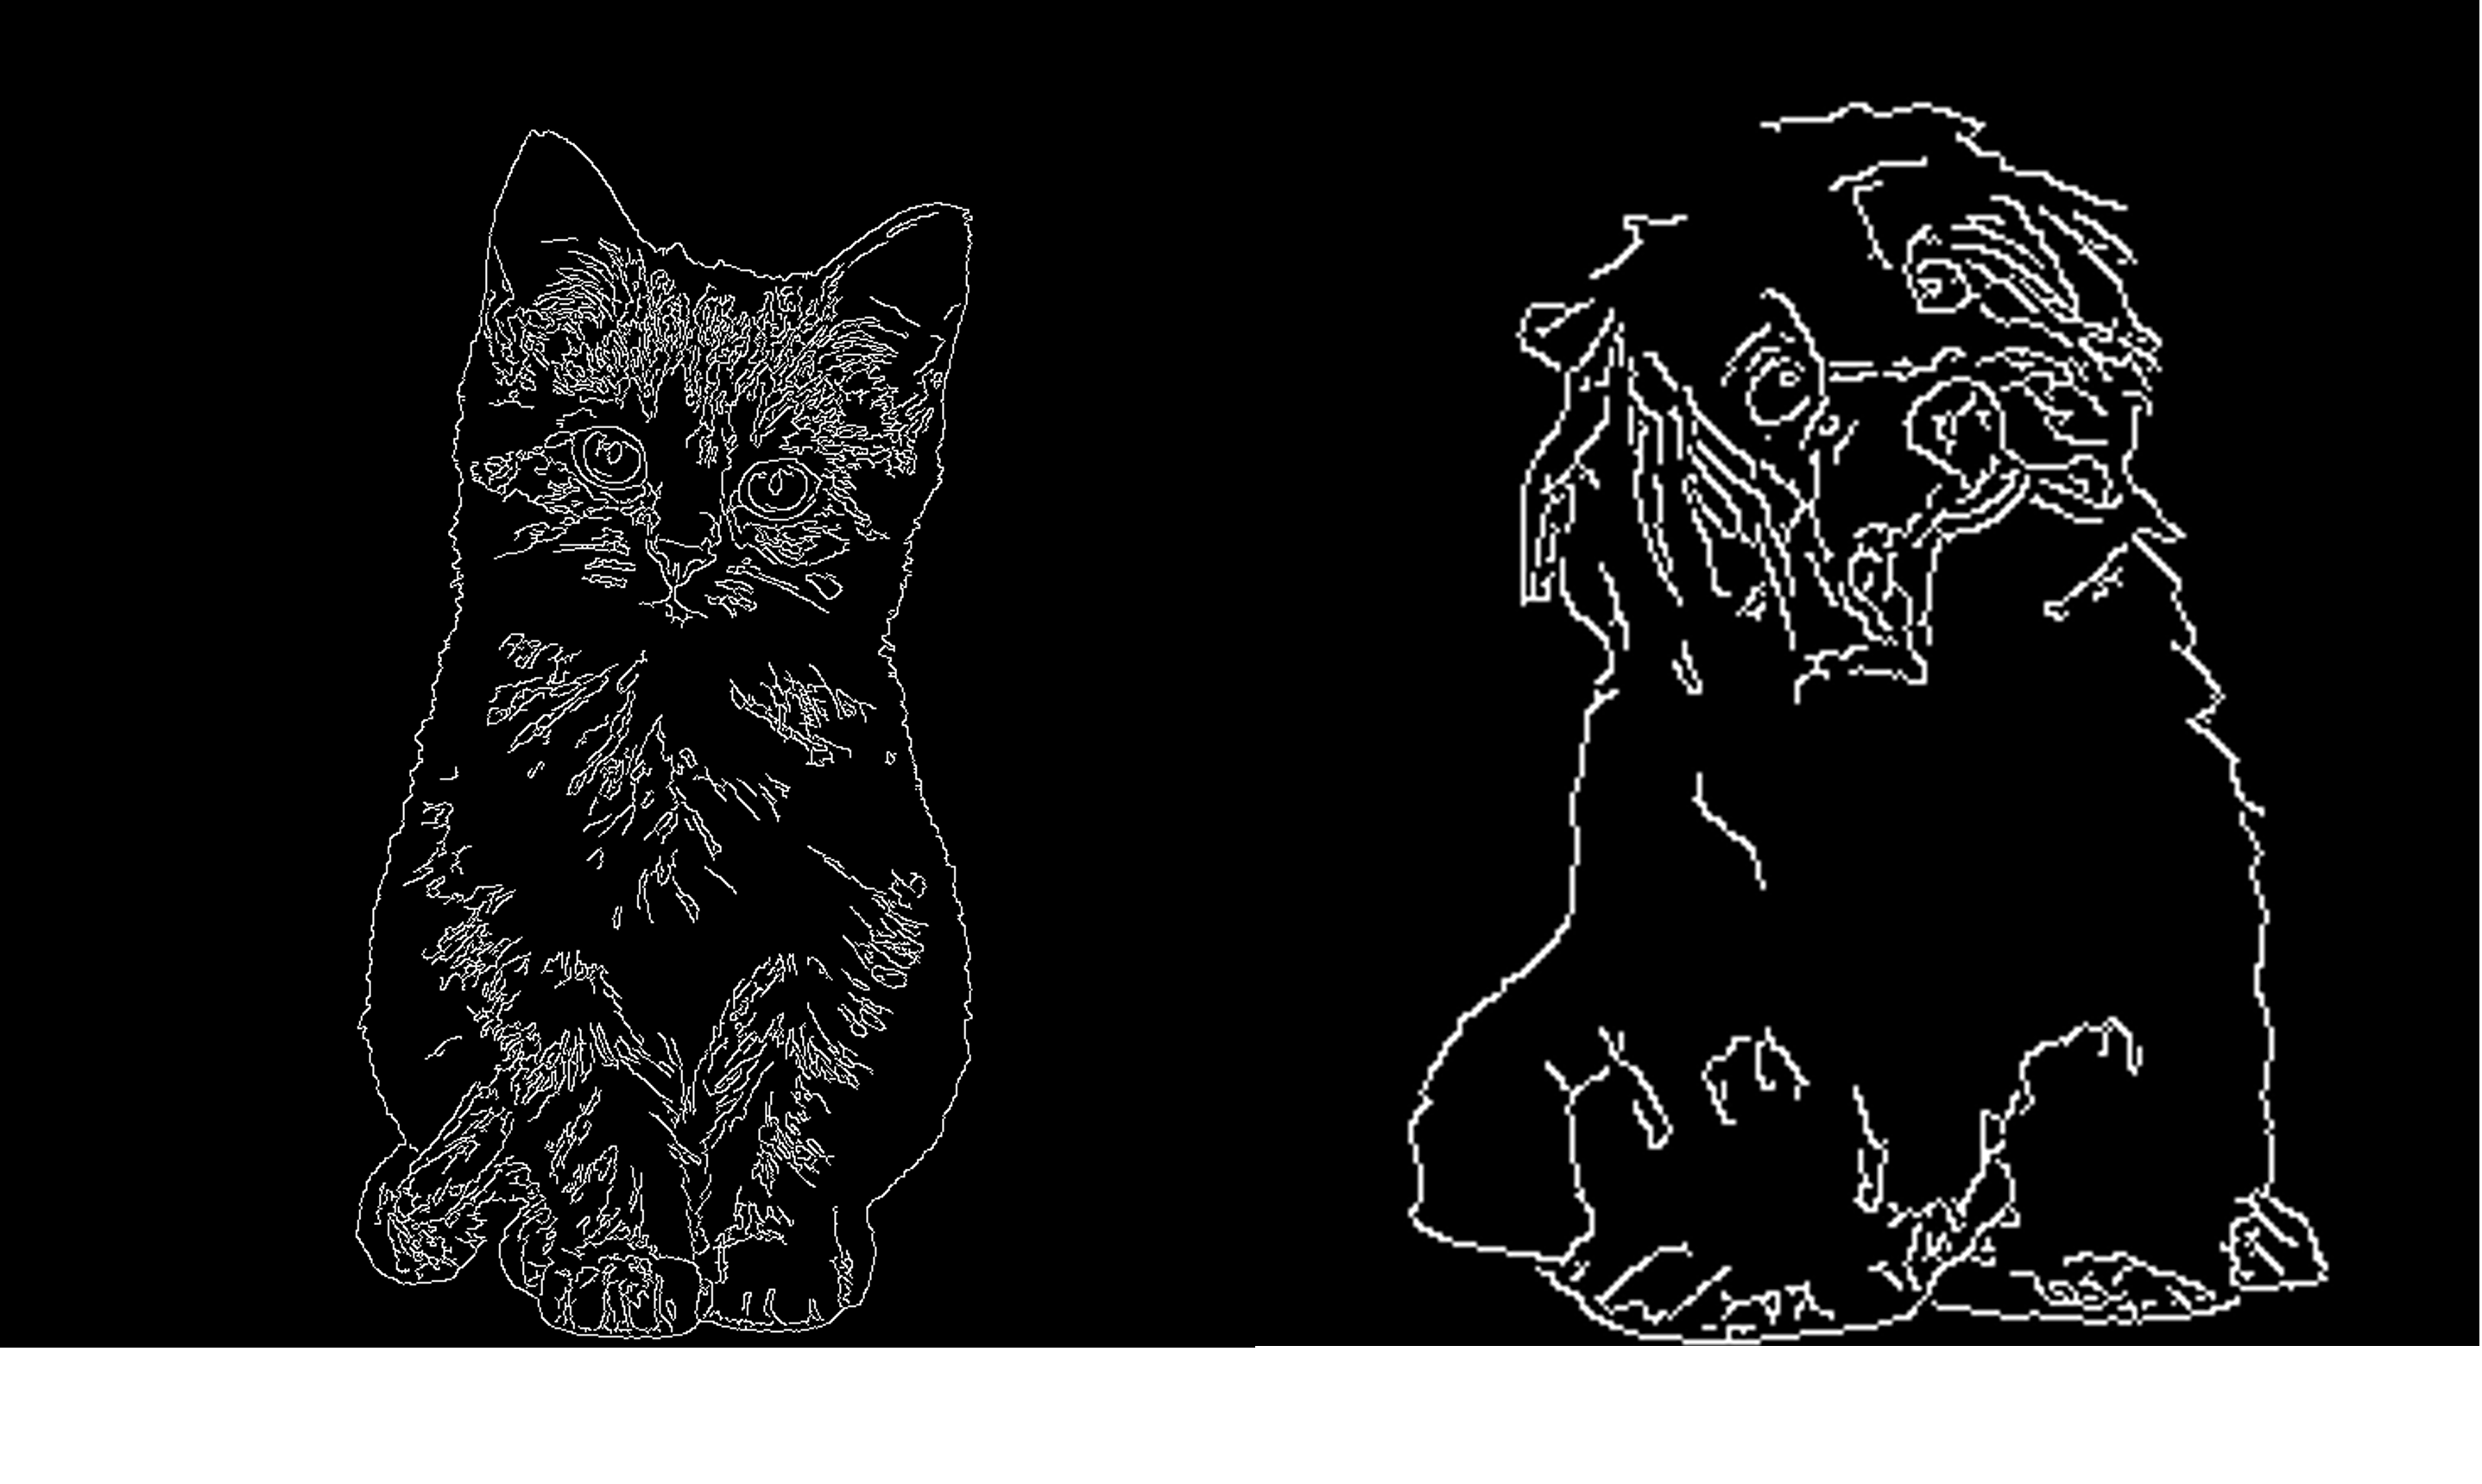
\includegraphics[width=\textwidth,height=\textheight,keepaspectratio]{CatDog_edge.png}%
    % \includegraphics[width=0.475\textwidth]{Dog_edge.png}
\end{frame}
% \begin{frame}[fragile]{Intro to Machine Learning}
%     \textbf{Why Machine Learning?}
%     \href{https://www.youtube.com/playlist?list=PLe3zogoPd5DY07OpTP4nFNOdMqItwtgc2}{Videos}.
% \end{frame}
\begin{frame}[fragile]{Intro to Machine Learning}
    \textbf{Why Machine Learning?}
    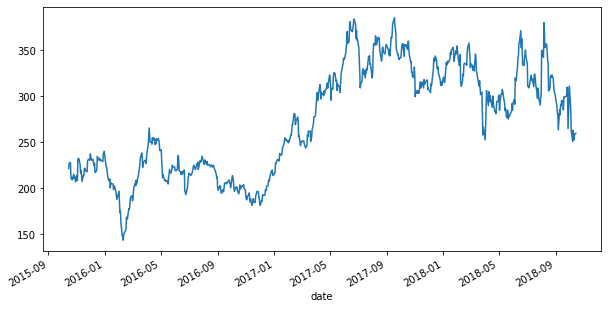
\includegraphics[width=\textwidth,height=\textheight,keepaspectratio]{Stock_block.png}
\end{frame}
\begin{frame}[fragile]{Intro to Machine Learning}
    \textbf{Why Machine Learning?}
    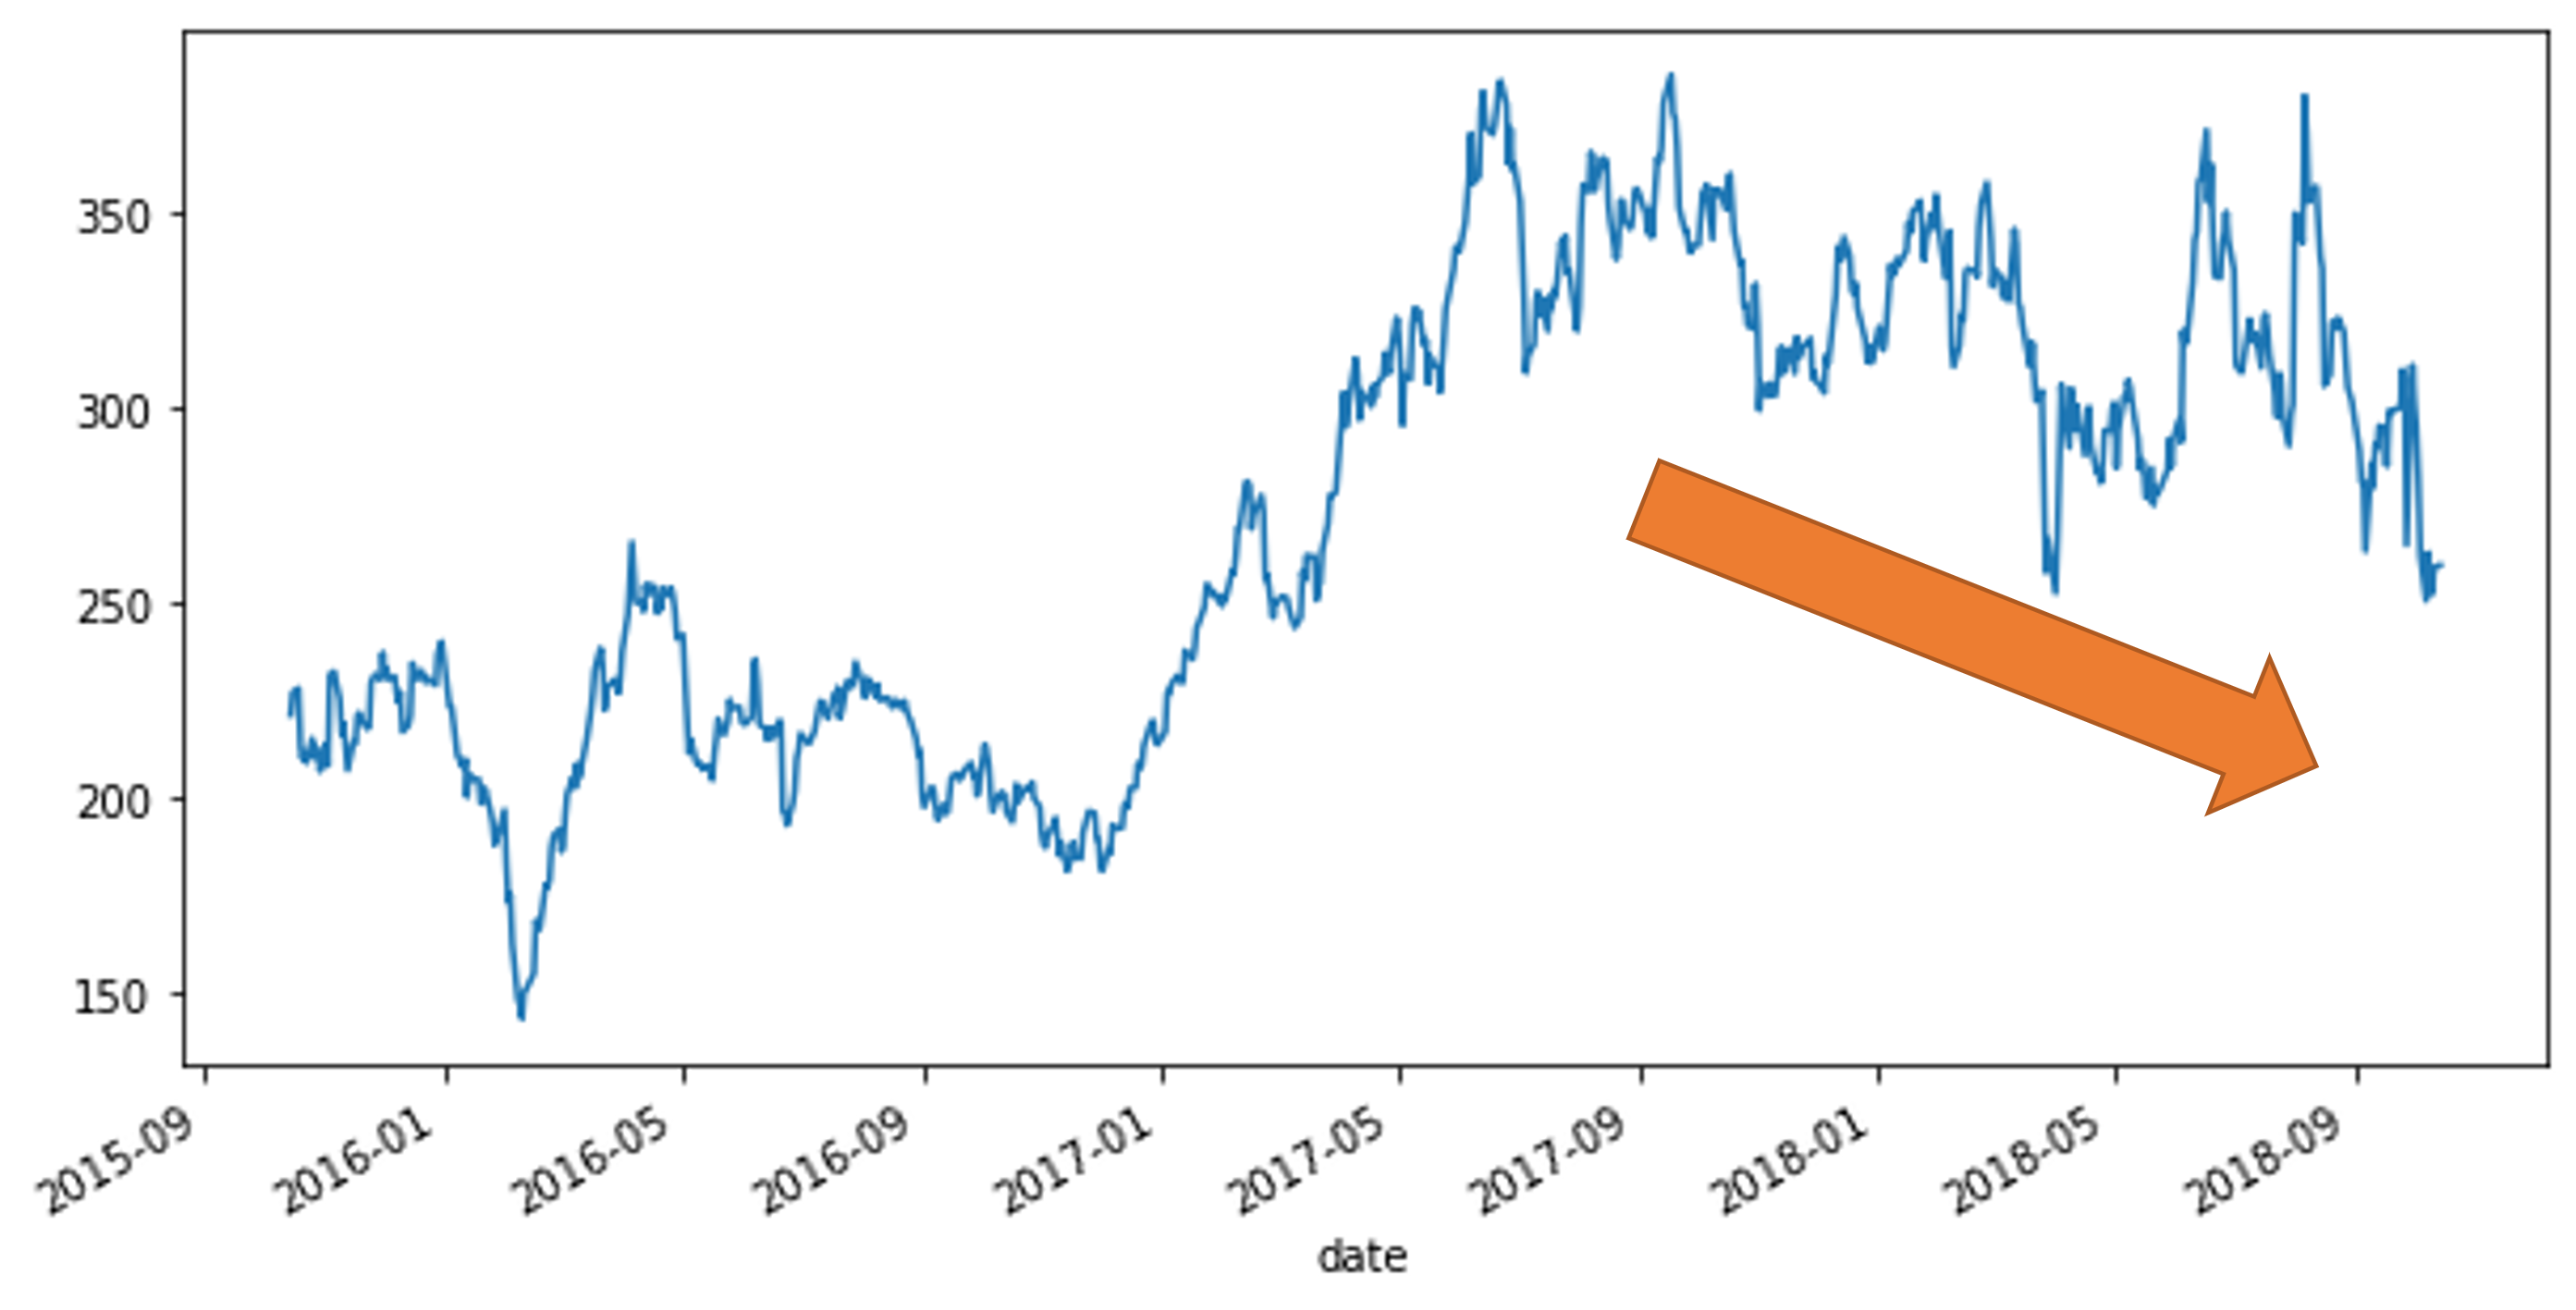
\includegraphics[width=\textwidth,height=\textheight,keepaspectratio]{Stock_trend.png}
\end{frame}
\begin{frame}[fragile]{Intro to Machine Learning}
    \textbf{Why Machine Learning?}
    \begin{center}
        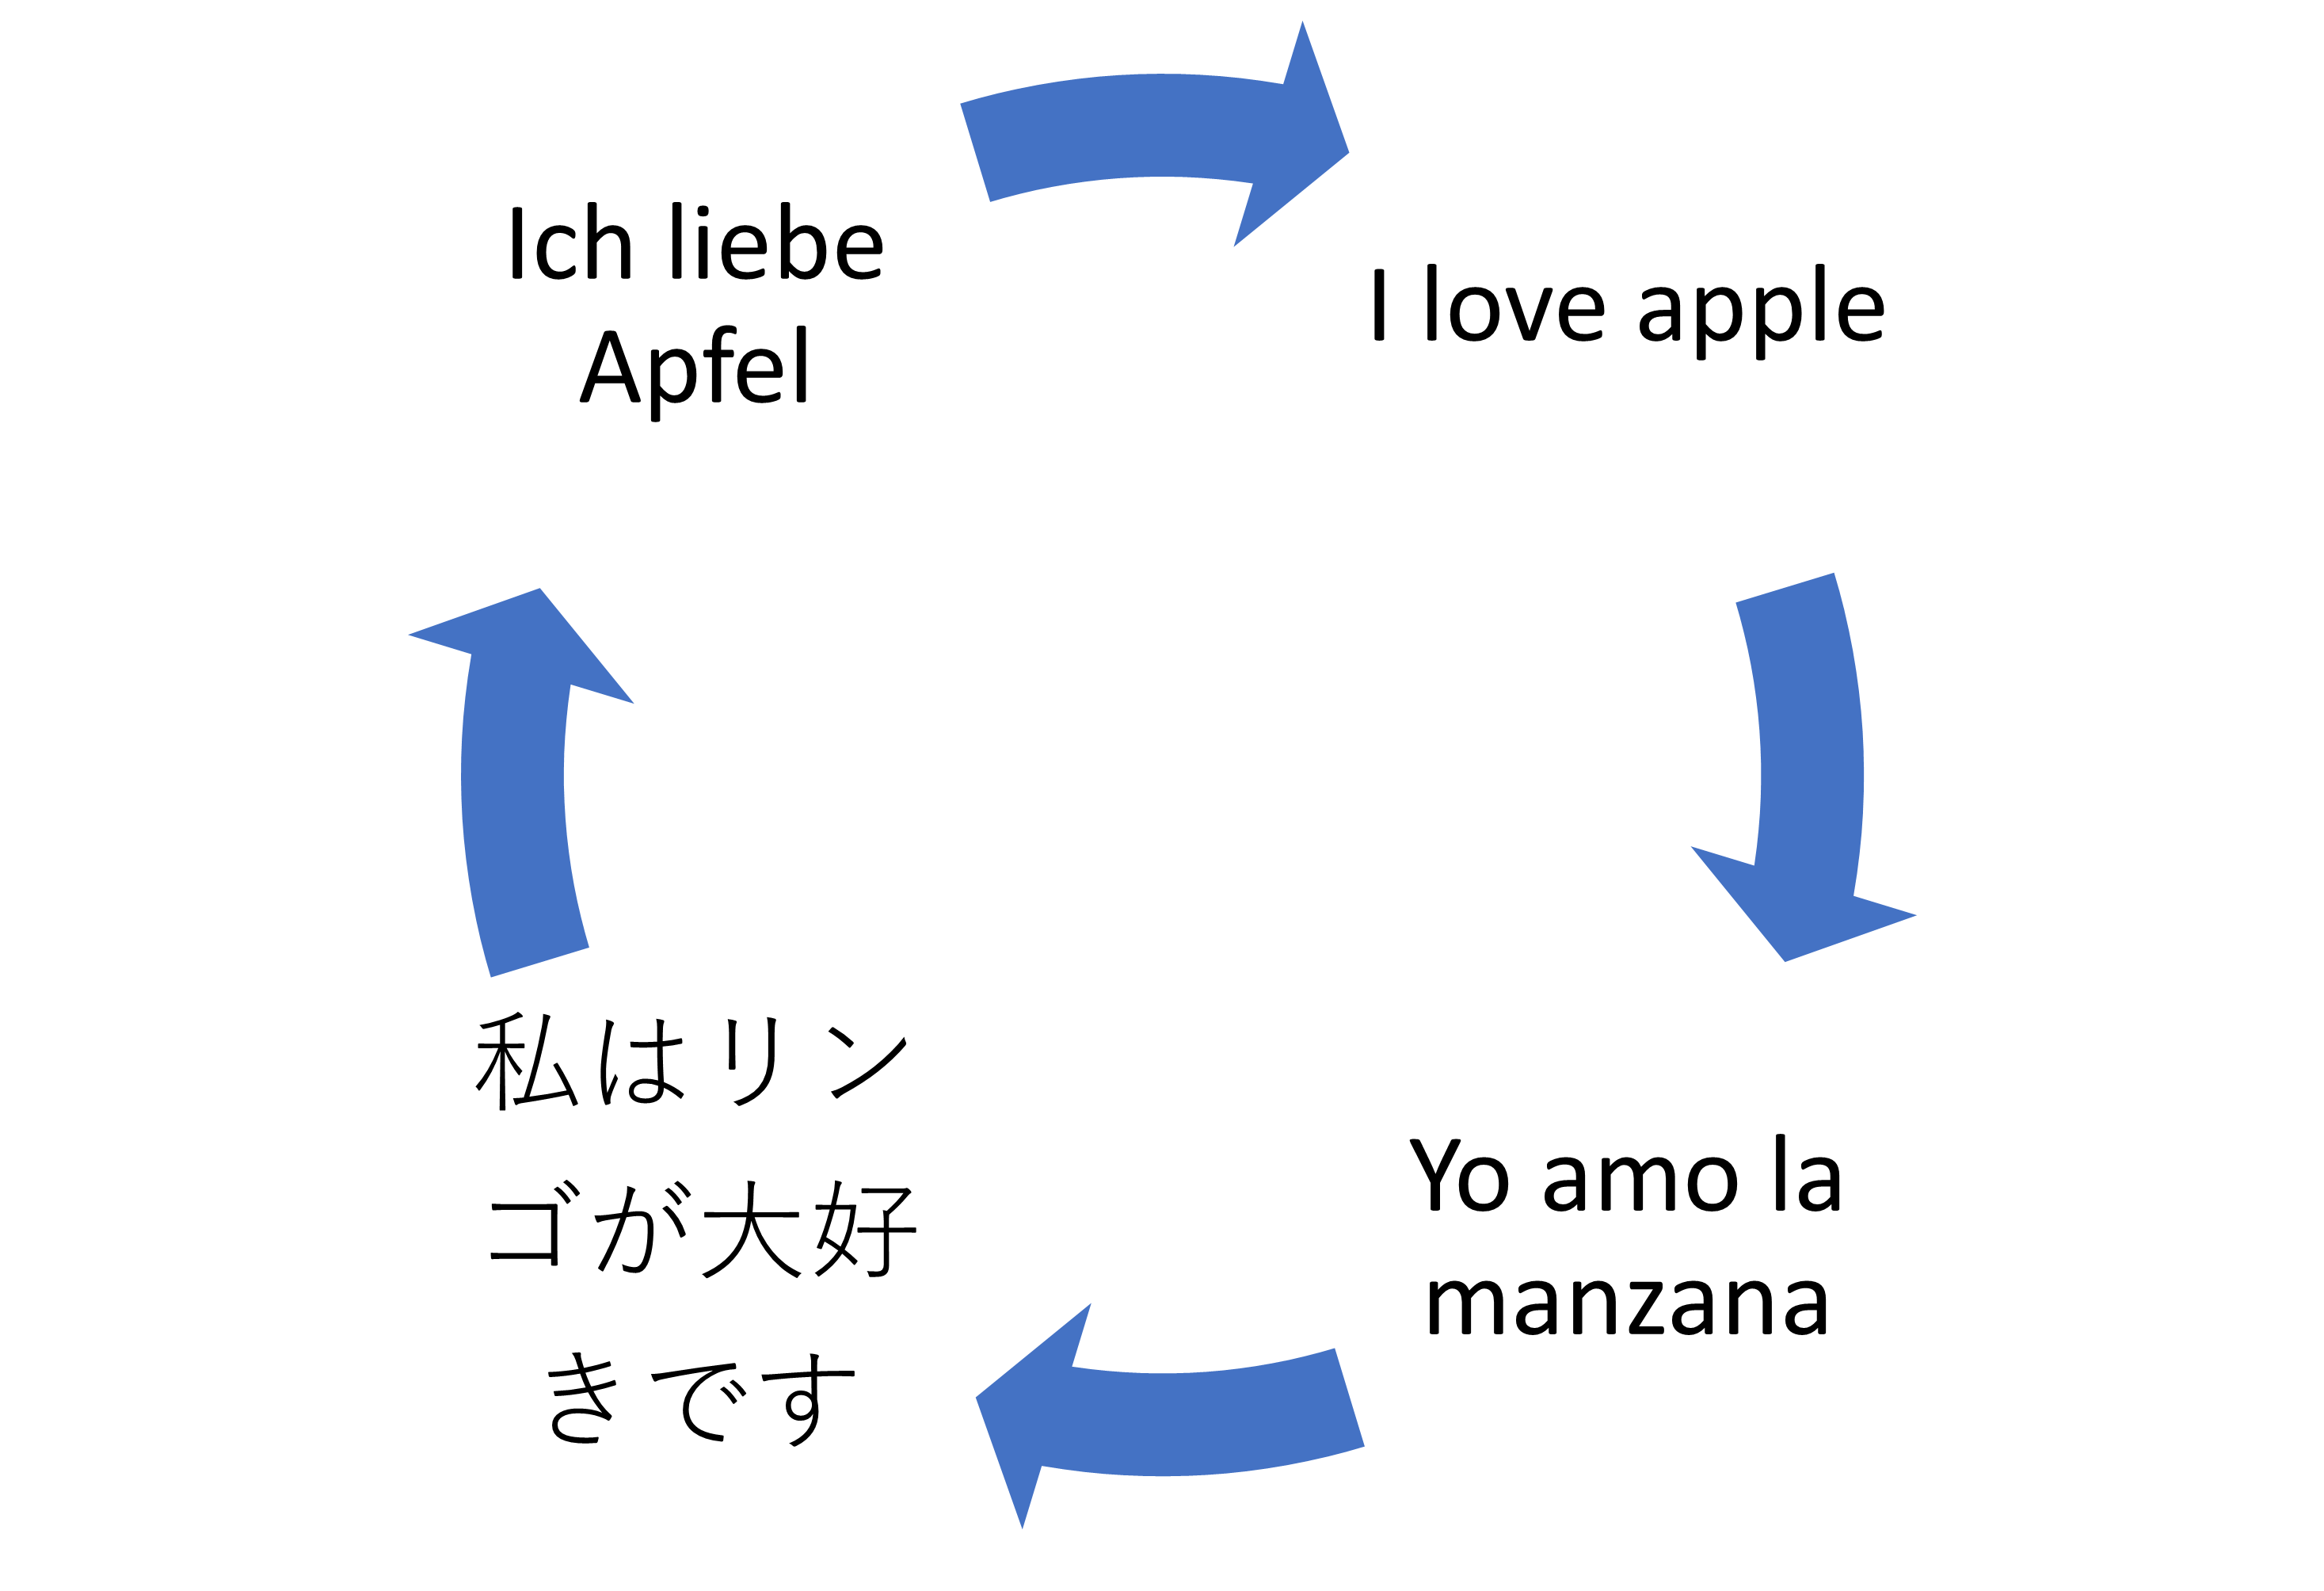
\includegraphics[width=\textwidth,height=0.8\textheight,keepaspectratio]{Lang_1.png}
    \end{center}
\end{frame}
\begin{frame}[fragile]{Intro to Machine Learning}
    \textbf{Why Machine Learning?}
    \begin{center}
        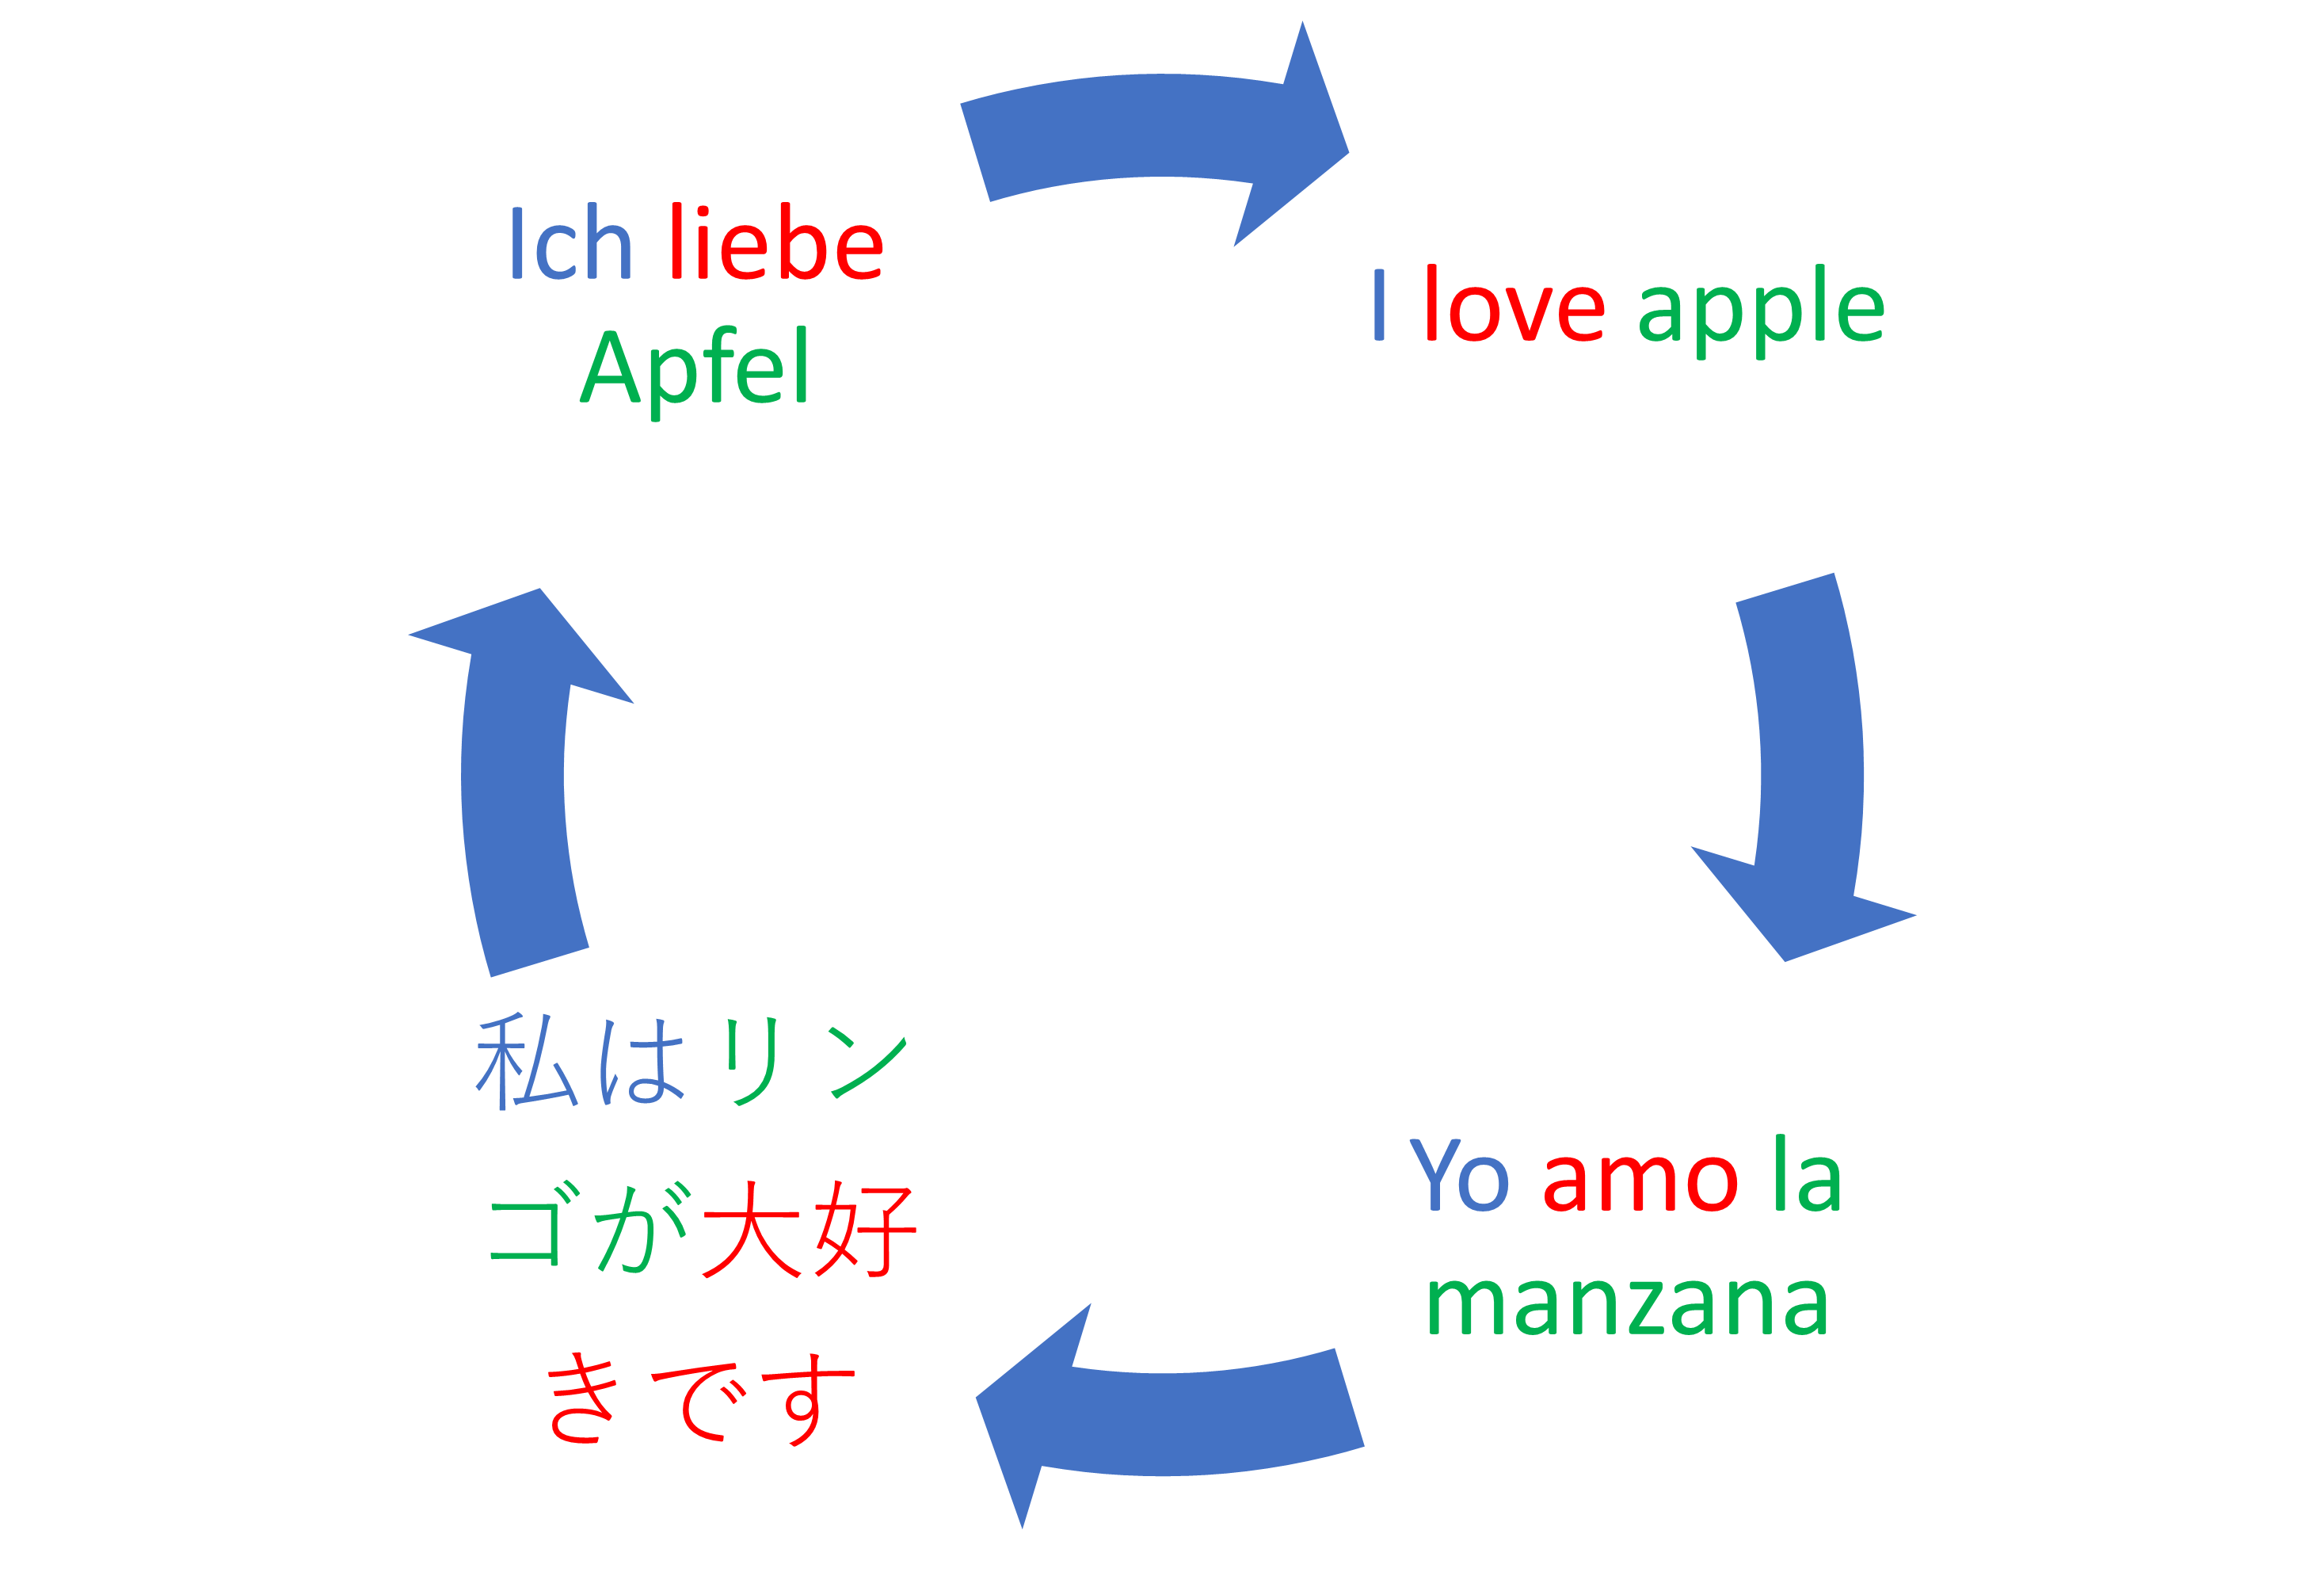
\includegraphics[width=\textwidth,height=0.8\textheight,keepaspectratio]{Lang_2.png}
    \end{center}
\end{frame}

\begin{frame}[fragile]{Intro to Machine Learning}
    \begin{block}{What is Machine Learning?}
        \begin{itemize}
            \item A cross-discipline field of study that combines aspects of Data Science, Data Engineering, Statistics and Probabilities, and Computer Programming to model highly complex functions.
            \pause
            \item 90\% of the time is spent on cleaning and making the data work; 10\% of the time is spent on actual machine learning.
            \item \huge $f(x)$
        \end{itemize}
    \end{block}
\end{frame}
\begin{frame}[fragile]{Intro to Machine Learning}
    \textbf{What is Machine Learning?}
    \begin{block}{Artificial Intelligence}
        \textbf{Artificial Intelligence} is a question: How do we build systems that solve tasks for which humans need intelligence?
    \end{block}
    \begin{block}{Machine Learning}
        \textbf{Machine Learning} is the contemporary answer to the question: a set of techniques/algorithms that allow computers to learn to solve tasks from data.
    \end{block}
\end{frame}

\begin{frame}[fragile]{Intro to Machine Learning}
    \textbf{Types of Machine Learning task}
    \begin{itemize}
        \item Supervised Learning
        \item Unsupervised Learning
        \item Reinforcement Learning
    \end{itemize}
\end{frame}

\begin{frame}[fragile]{Intro to Machine Learning}
    \textbf{Supervised Learning}
    \begin{center}
        
\includegraphics[width=\textwidth,height=0.7\textheight,keepaspectratio]{Target.png}
    \end{center}
\end{frame}
\begin{frame}[fragile]{Intro to Machine Learning}
    \textbf{Supervised Learning}
    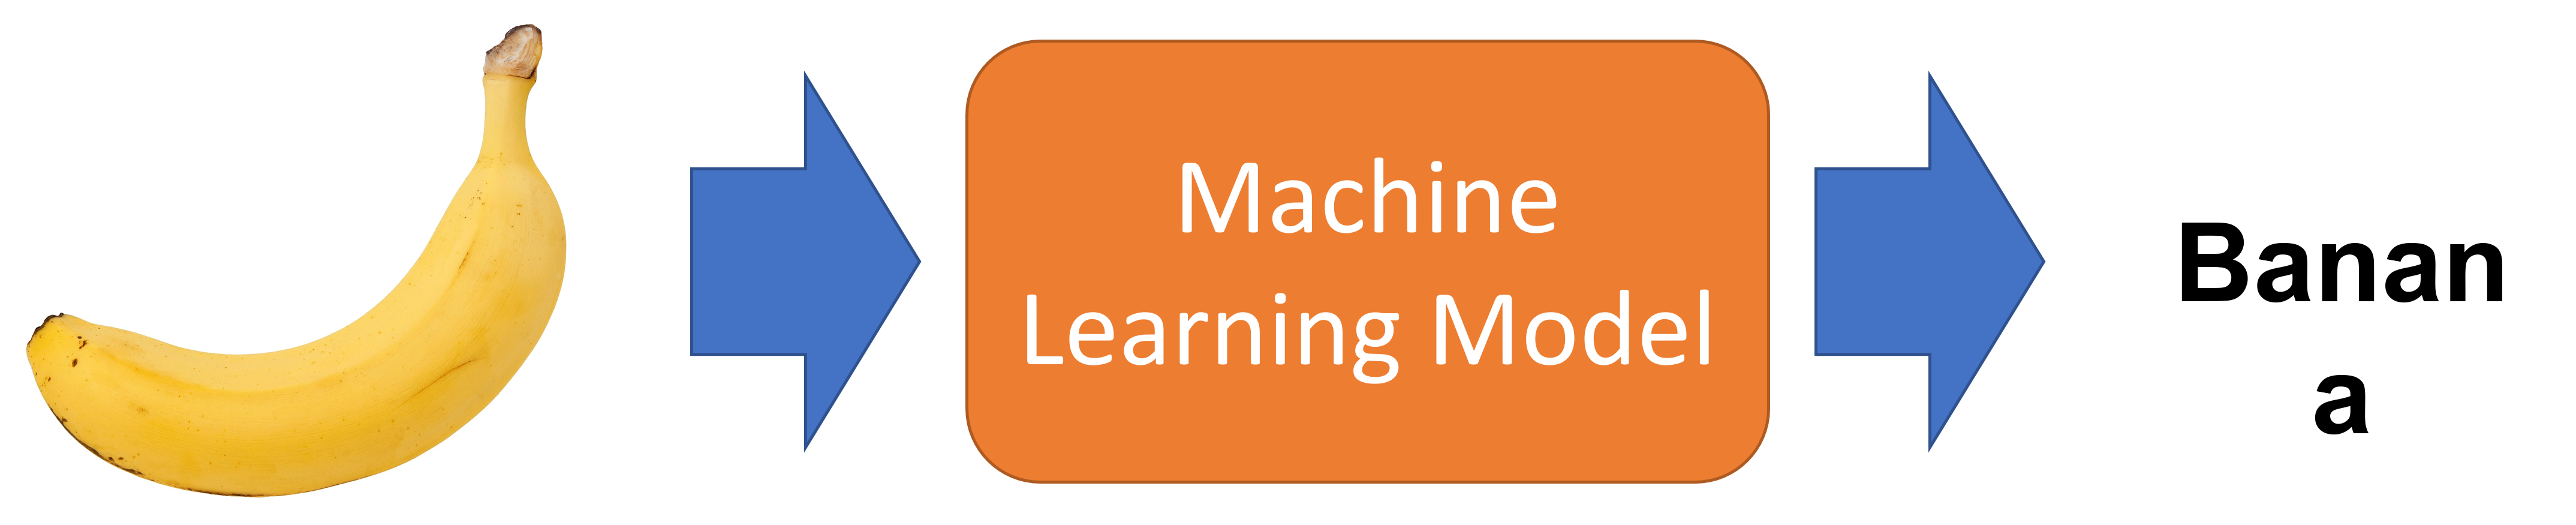
\includegraphics[width=\textwidth,height=\textheight,keepaspectratio]{Supervised_example_1.png}
\end{frame}
\begin{frame}[fragile]{Intro to Machine Learning}
    \textbf{Supervised Learning}
    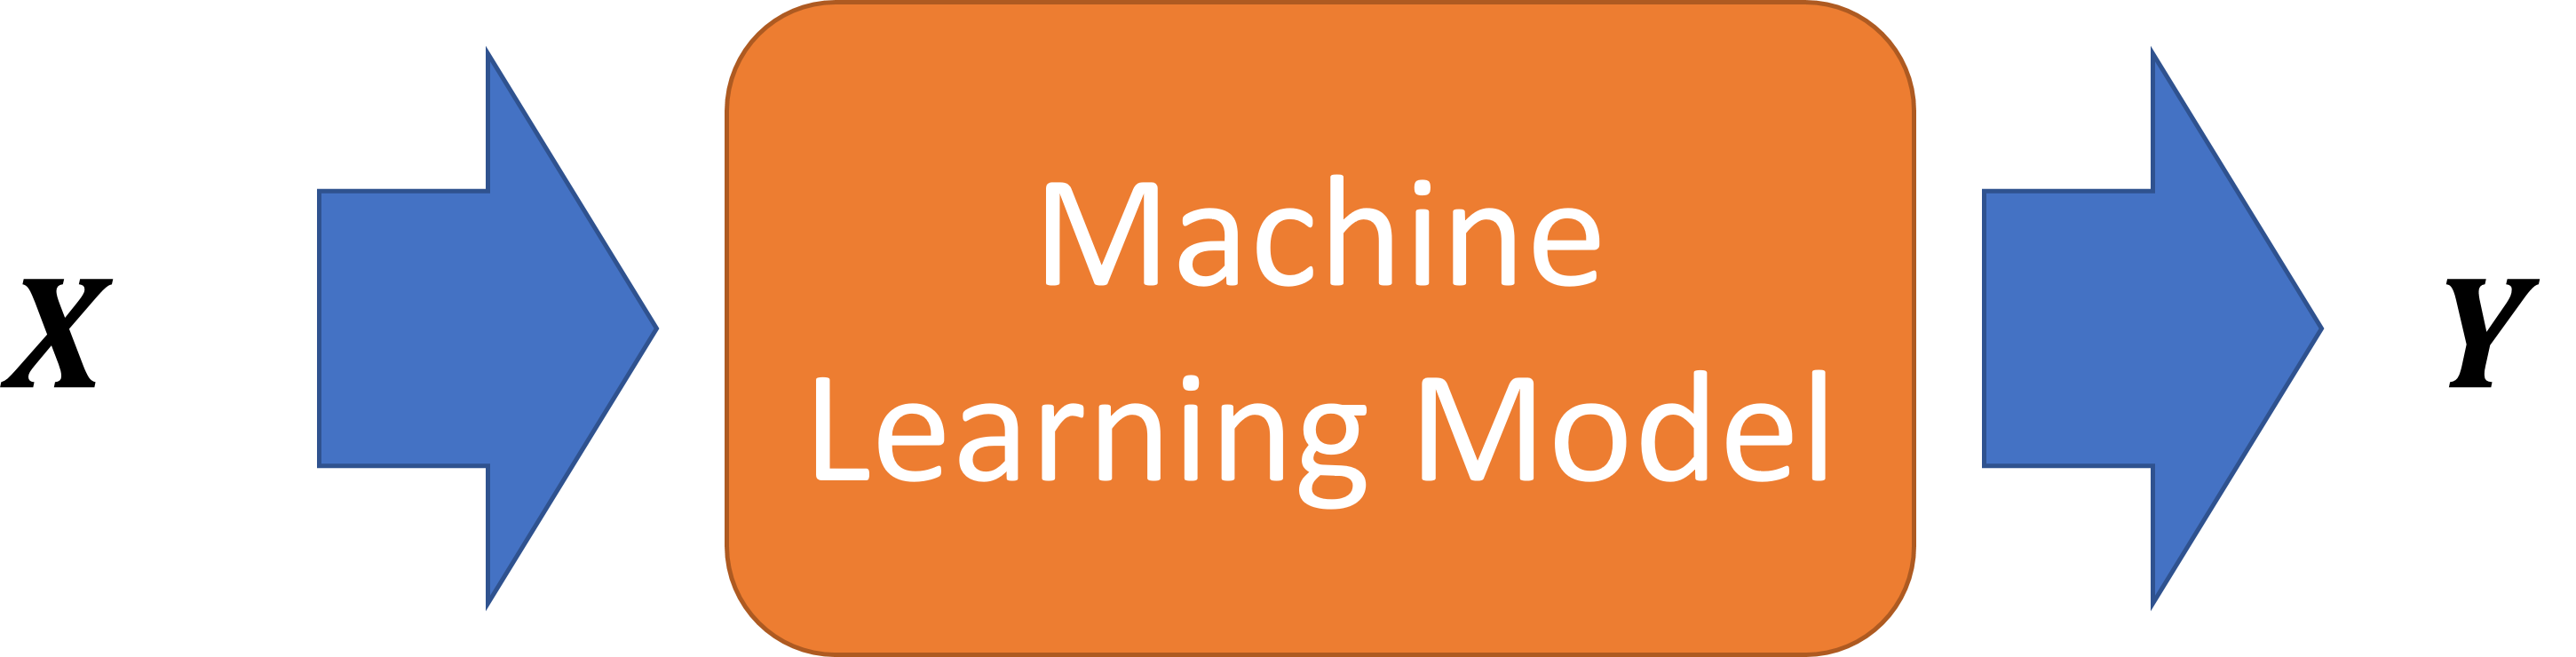
\includegraphics[width=\textwidth,height=\textheight,keepaspectratio]{Supervised.png}
\end{frame}
\begin{frame}[fragile]{Intro to Machine Learning}
    \textbf{Supervised Learning}
    \begin{itemize}
        \item is a machine learning paradigm that learns a mapping function between input and output data.
        \item needs pairs of input features and labelled output targets.
        \pause
        \item sensitive to target's noise and outliers.
        \item has a bias-variance dilemma.
        \item affected by the curse of dimensionality and complexity.
    \end{itemize}
\end{frame}

\begin{frame}[fragile]{Intro to Machine Learning}
    \textbf{Unsupervised Learning}
    \begin{center}
        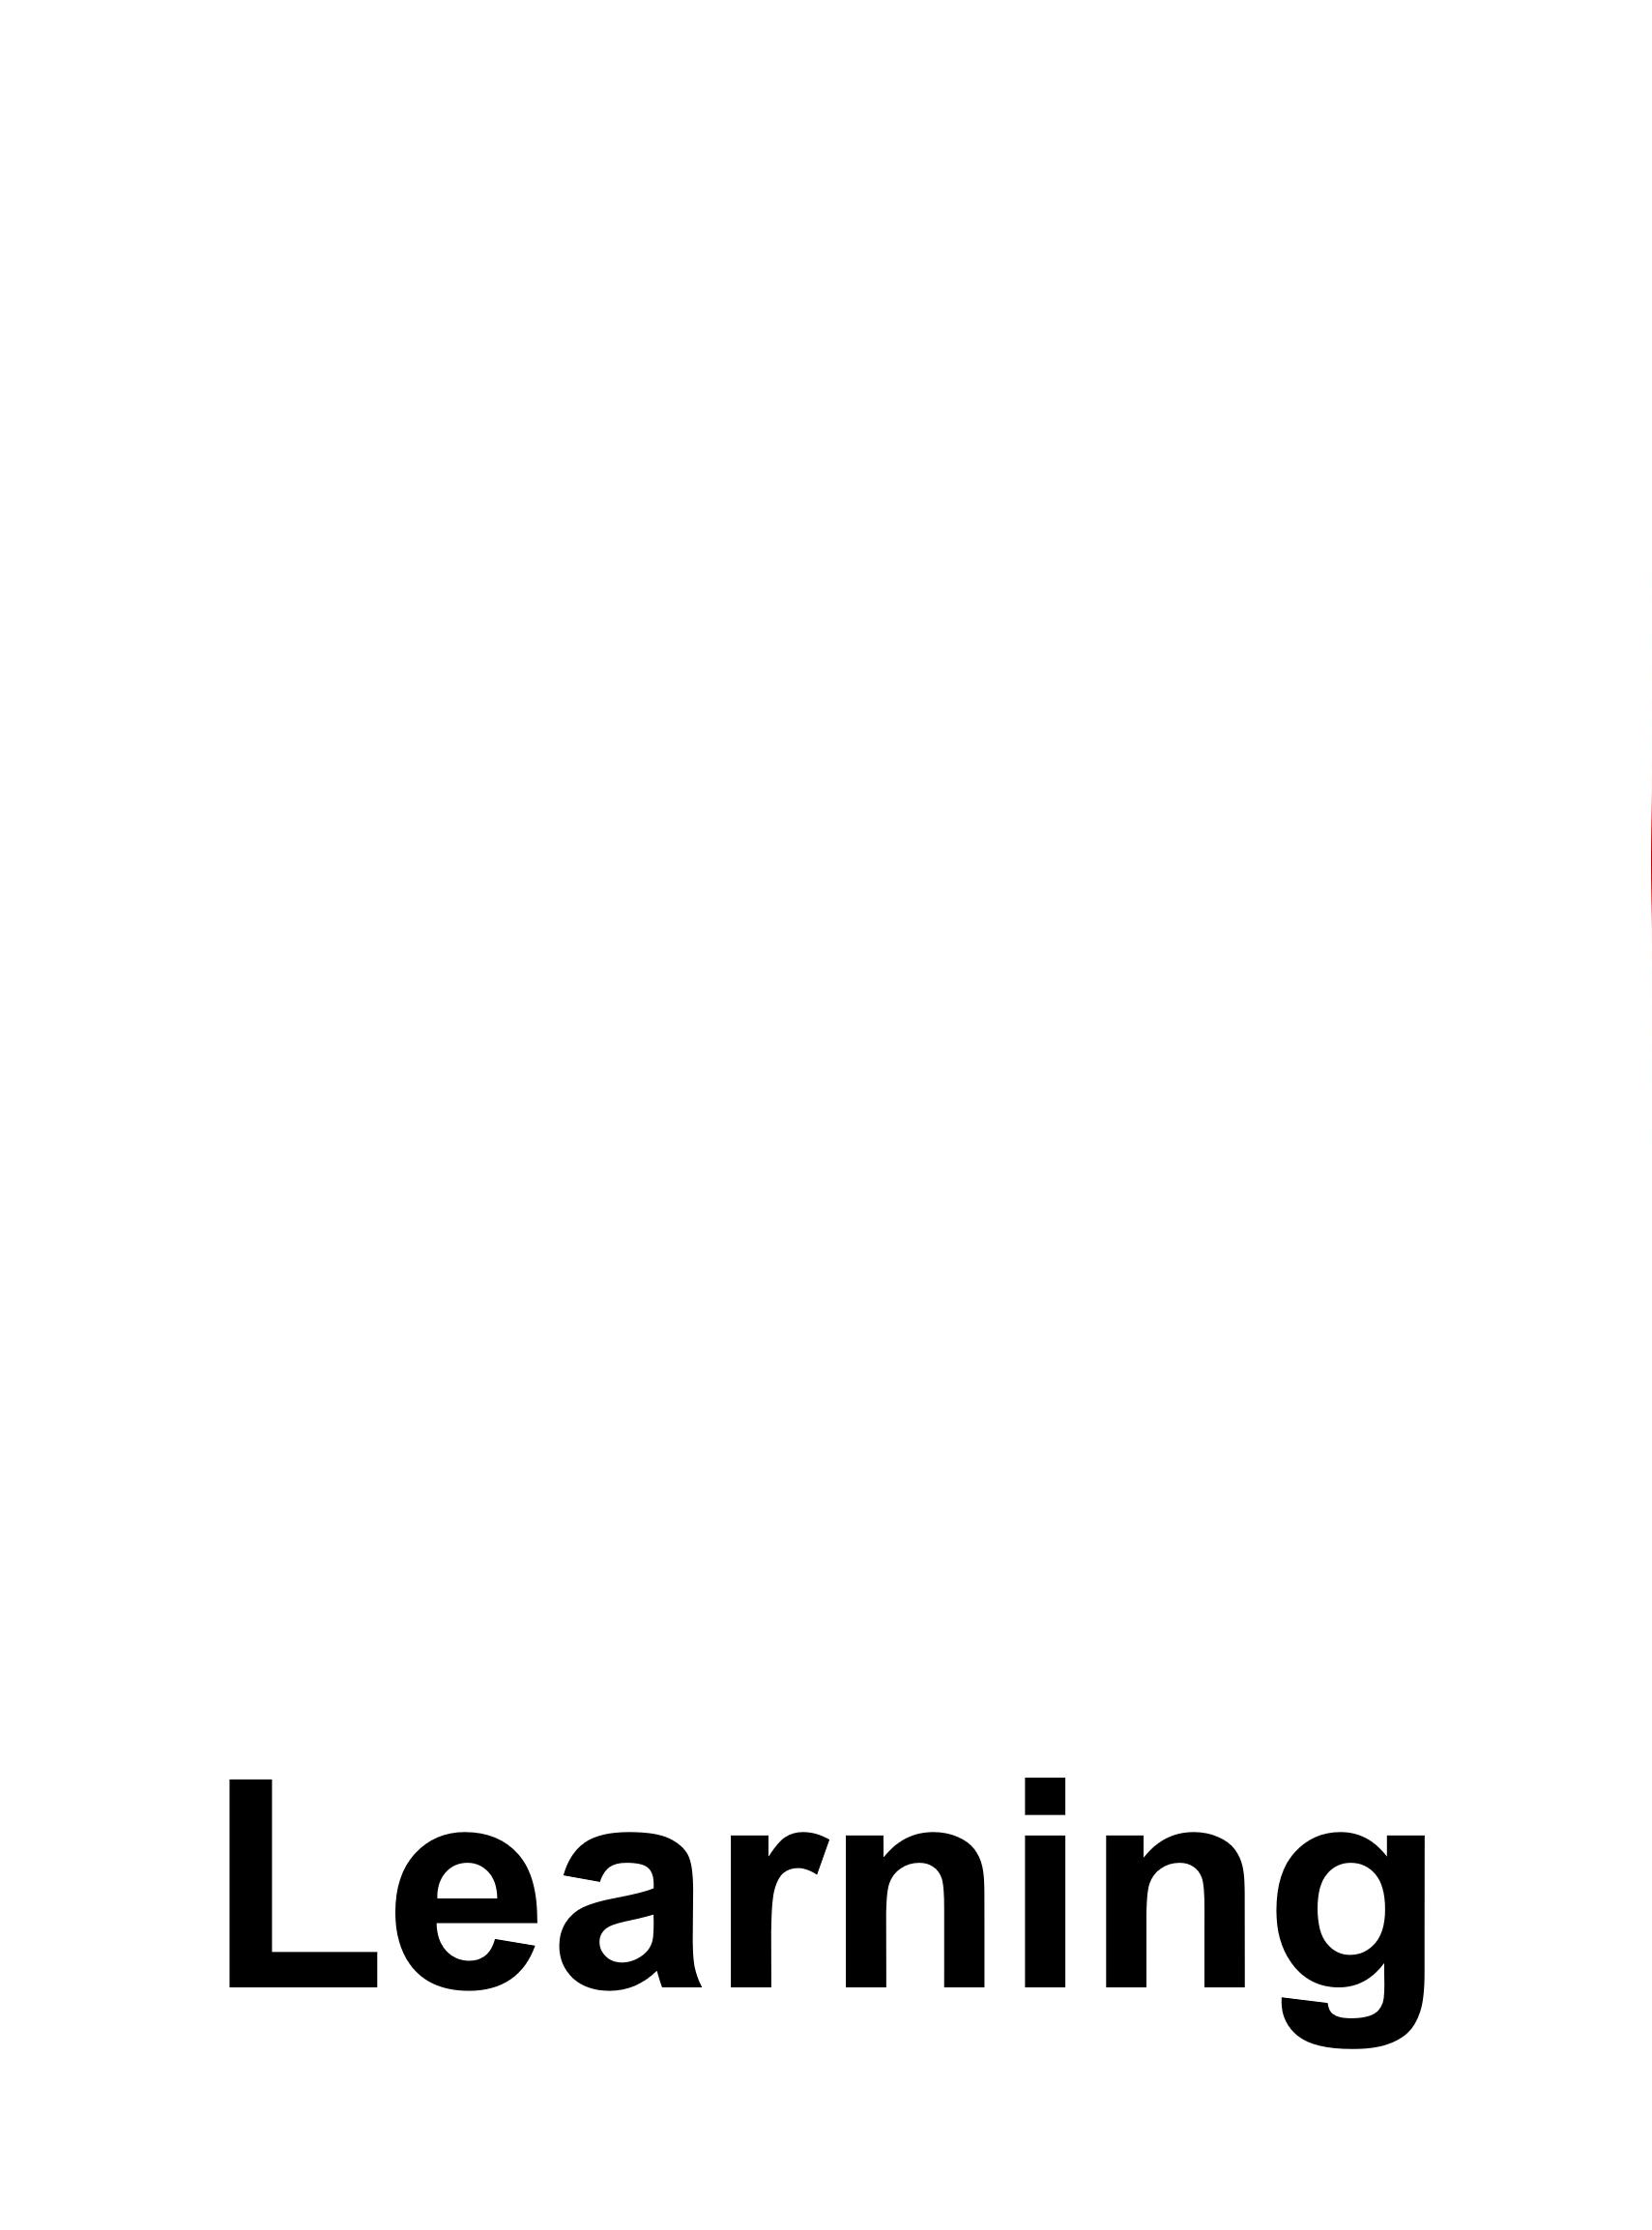
\includegraphics[width=\textwidth,height=0.7\textheight,keepaspectratio]{UnTarget.png}
    \end{center}
\end{frame}
\begin{frame}[fragile]{Intro to Machine Learning}
    \textbf{Unsupervised Learning}
    \includegraphics[width=\textwidth,height=\textheight,keepaspectratio]{Unsupervised_example.png}
\end{frame}
\begin{frame}[fragile]{Intro to Machine Learning}
    \textbf{Unsupervised Learning}
    \begin{center}
        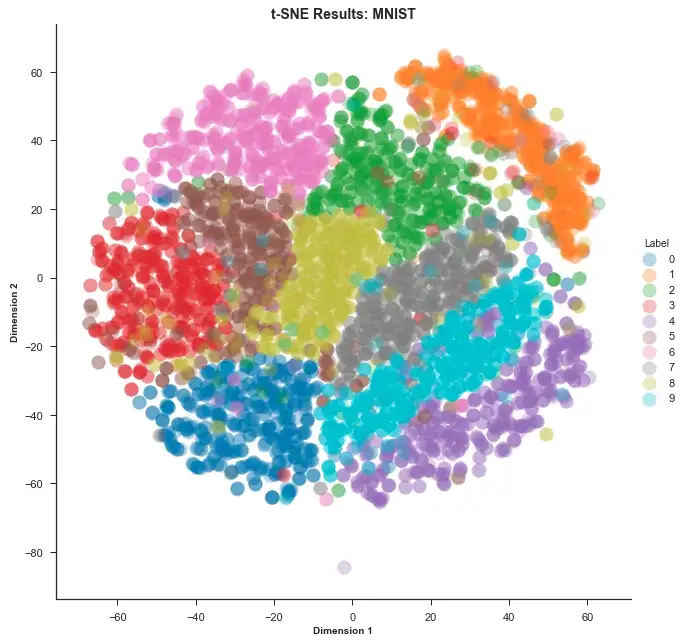
\includegraphics[width=\textwidth,height=0.7\textheight,keepaspectratio]{tSNE.png}
    \end{center}
\end{frame}
\begin{frame}[fragile]{Intro to Machine Learning}
    \textbf{Unsupervised Learning}
    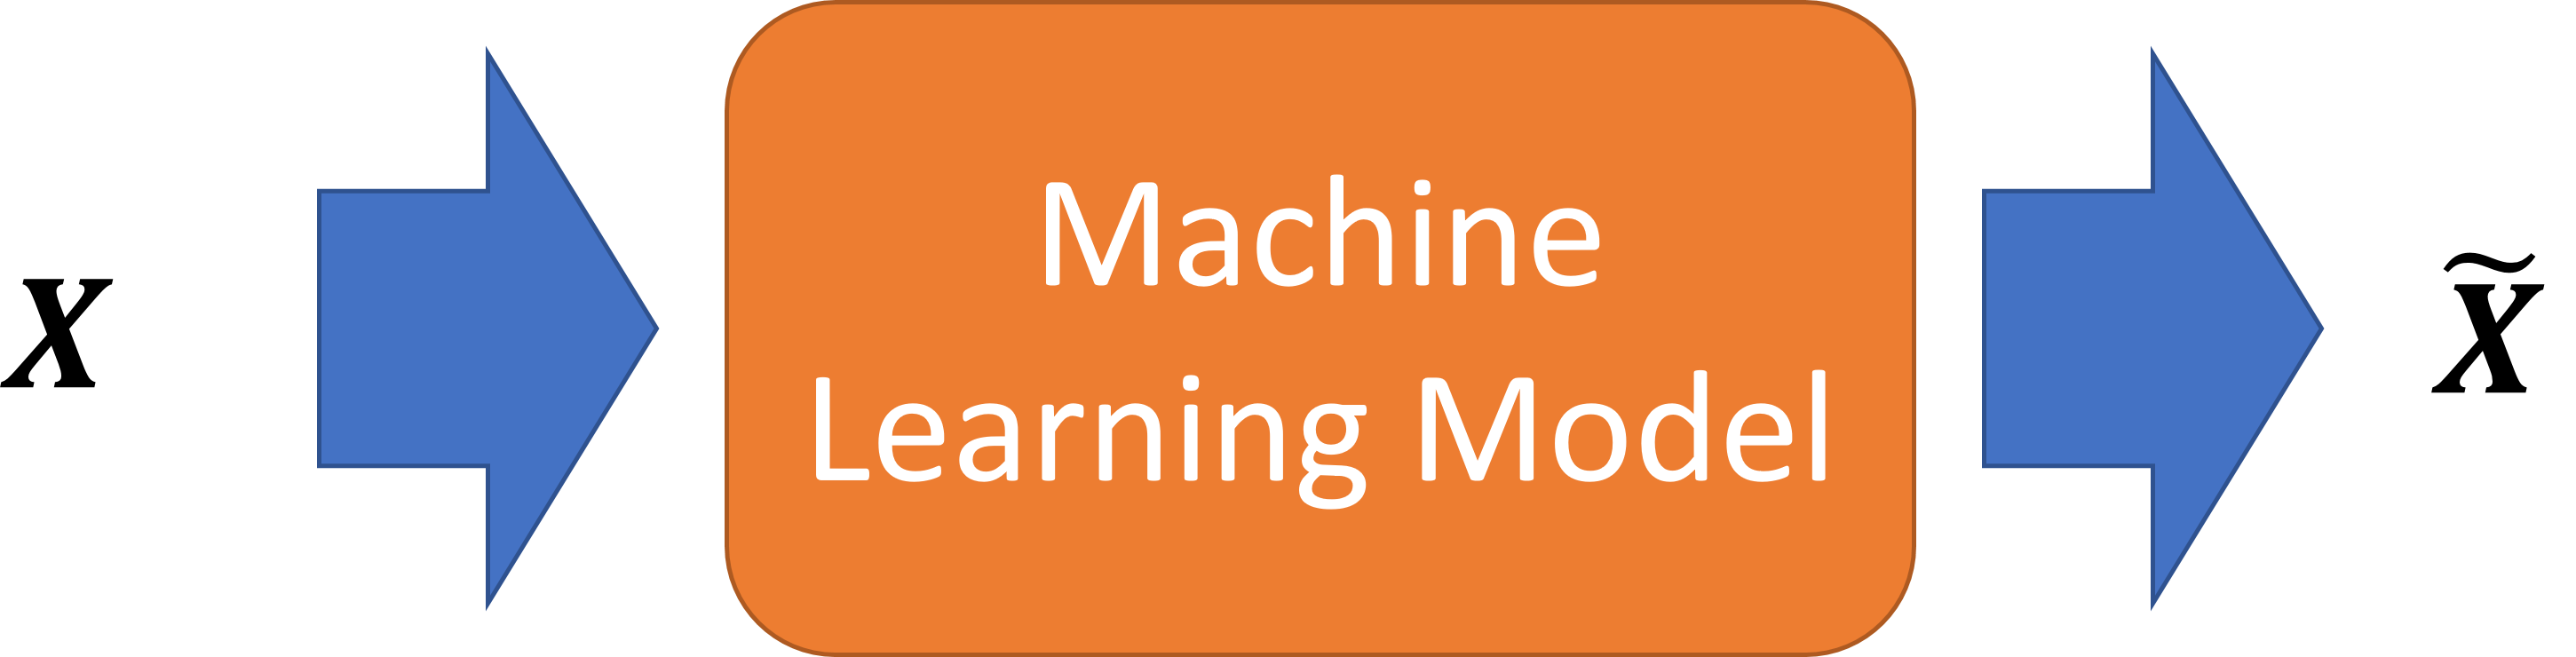
\includegraphics[width=\textwidth,height=\textheight,keepaspectratio]{Unsupervised.png}
\end{frame}
\begin{frame}[fragile]{Intro to Machine Learning}
    \textbf{Unsupervised Learning}
    \begin{itemize}
        \item is a machine learning paradigm that learns underlying patterns from input data.
        \item usually performs clustering and dimensional reduction.
        \pause
        \item sensitive to input's noise and outliers.
        \item has a bias-variance dilemma.
        \item Less accurate than supervised learning.
    \end{itemize}
\end{frame}

\begin{frame}[fragile]{Intro to Machine Learning}
    \textbf{Reinforcement Learning}
    \begin{center}
        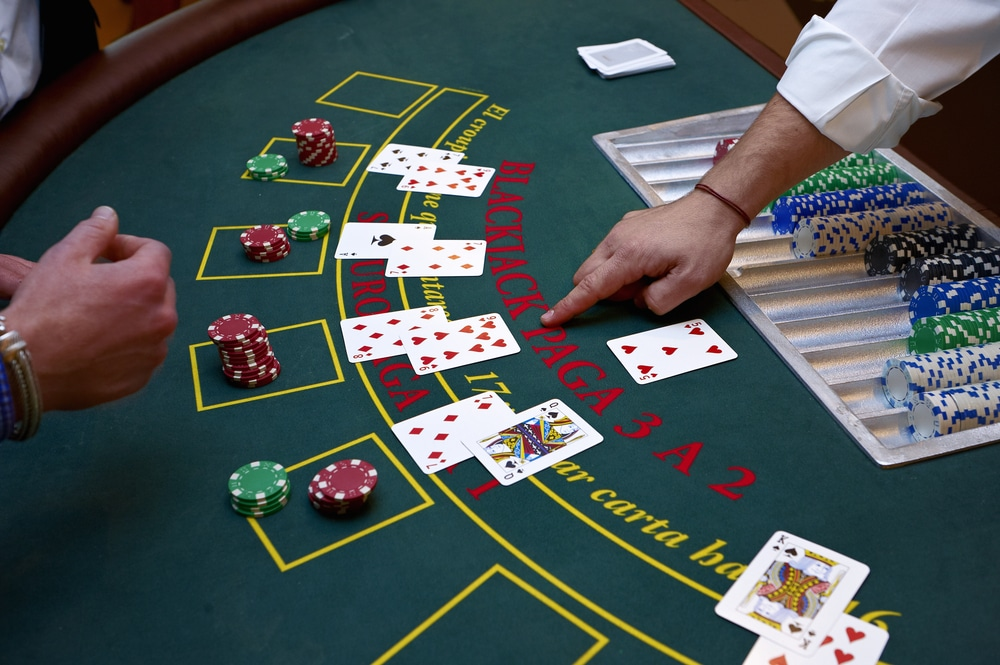
\includegraphics[width=\textwidth,height=0.7\textheight,keepaspectratio]{Blackjack.jpg}
    \end{center}
\end{frame}
\begin{frame}[fragile]{Intro to Machine Learning}
    \textbf{Reinforcement Learning}
    \begin{center}
        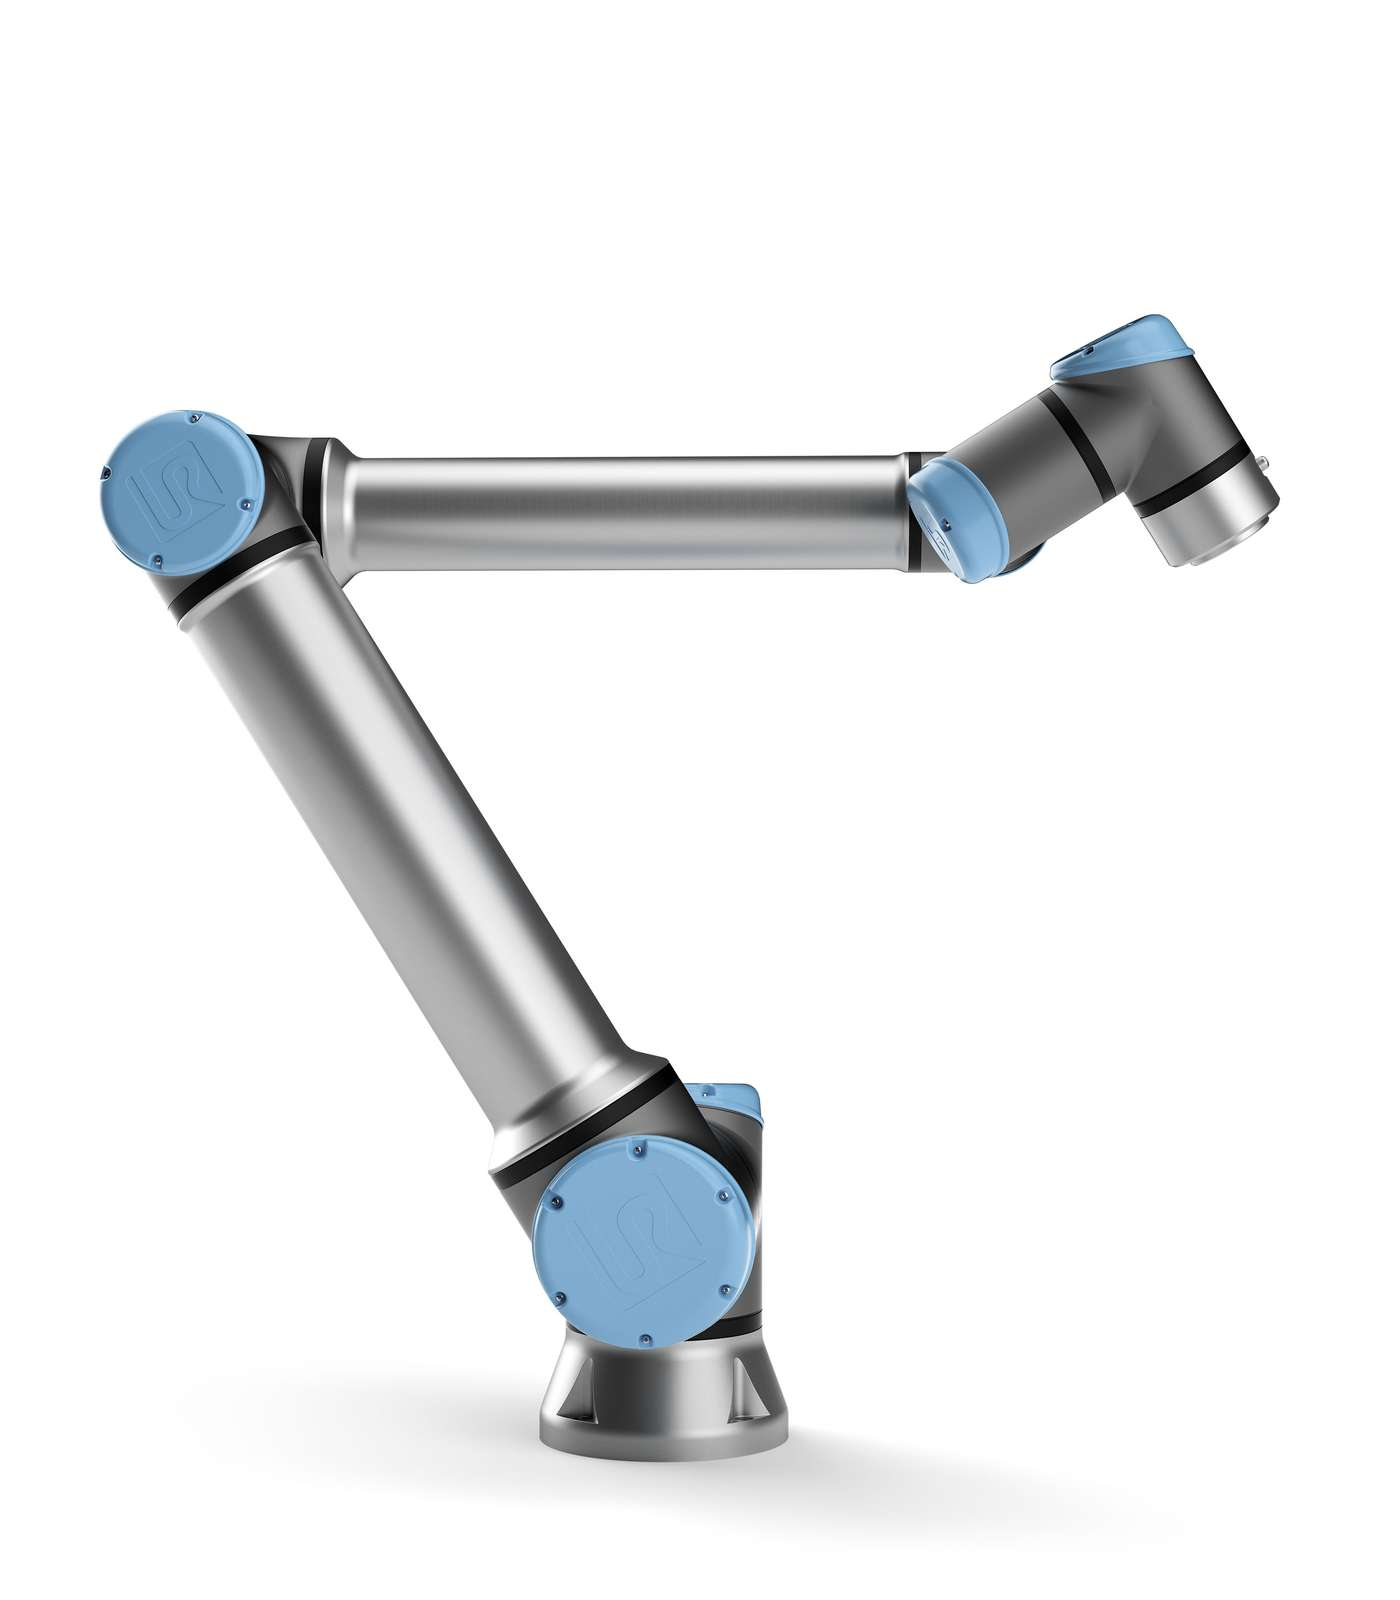
\includegraphics[width=\textwidth,height=0.7\textheight,keepaspectratio]{UR10e.jpg}
    \end{center}
\end{frame}
\begin{frame}[fragile]{Intro to Machine Learning}
    \textbf{Reinforcement Learning}
    \begin{center}
        \includegraphics[width=\textwidth,height=\textheight,keepaspectratio]{High-Jump.png}
    \end{center}
\end{frame}
\begin{frame}[fragile]{Intro to Machine Learning}
    \textbf{Reinforcement Learning}
    \begin{center}
        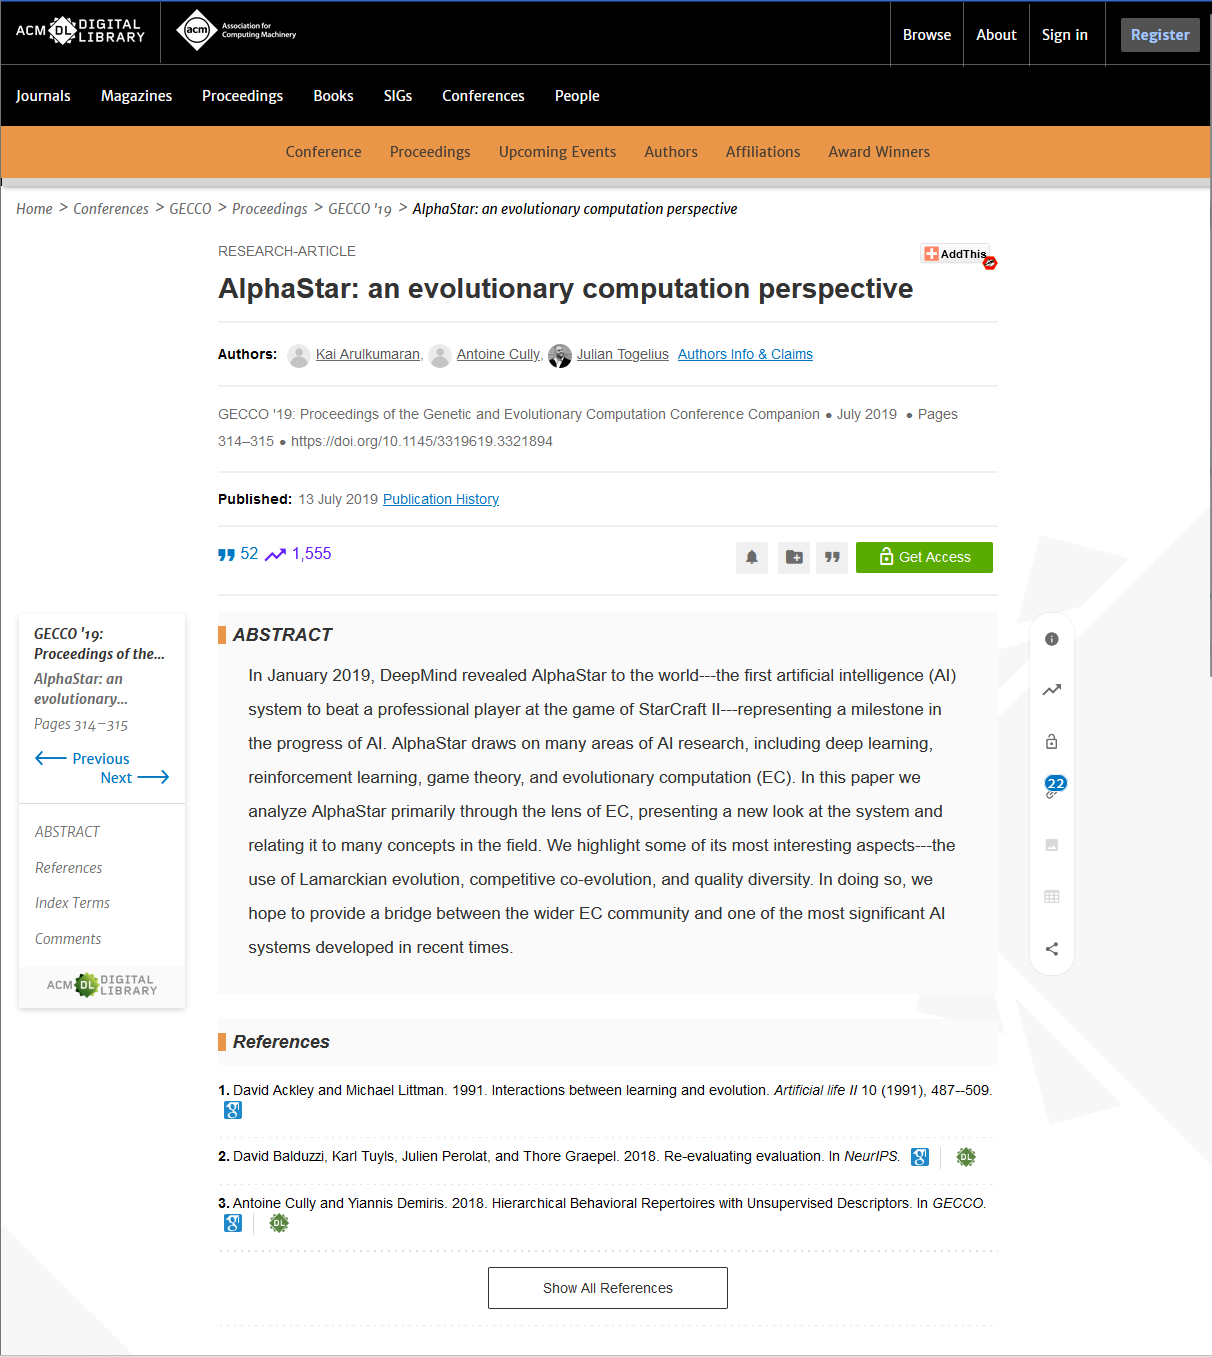
\includegraphics[width=\textwidth,height=0.7\textheight,keepaspectratio]{AlphaStar.png}
    \end{center}
\end{frame}
\begin{frame}[fragile]{Intro to Machine Learning}
    \textbf{Reinforcement Learning}
    \begin{center}
        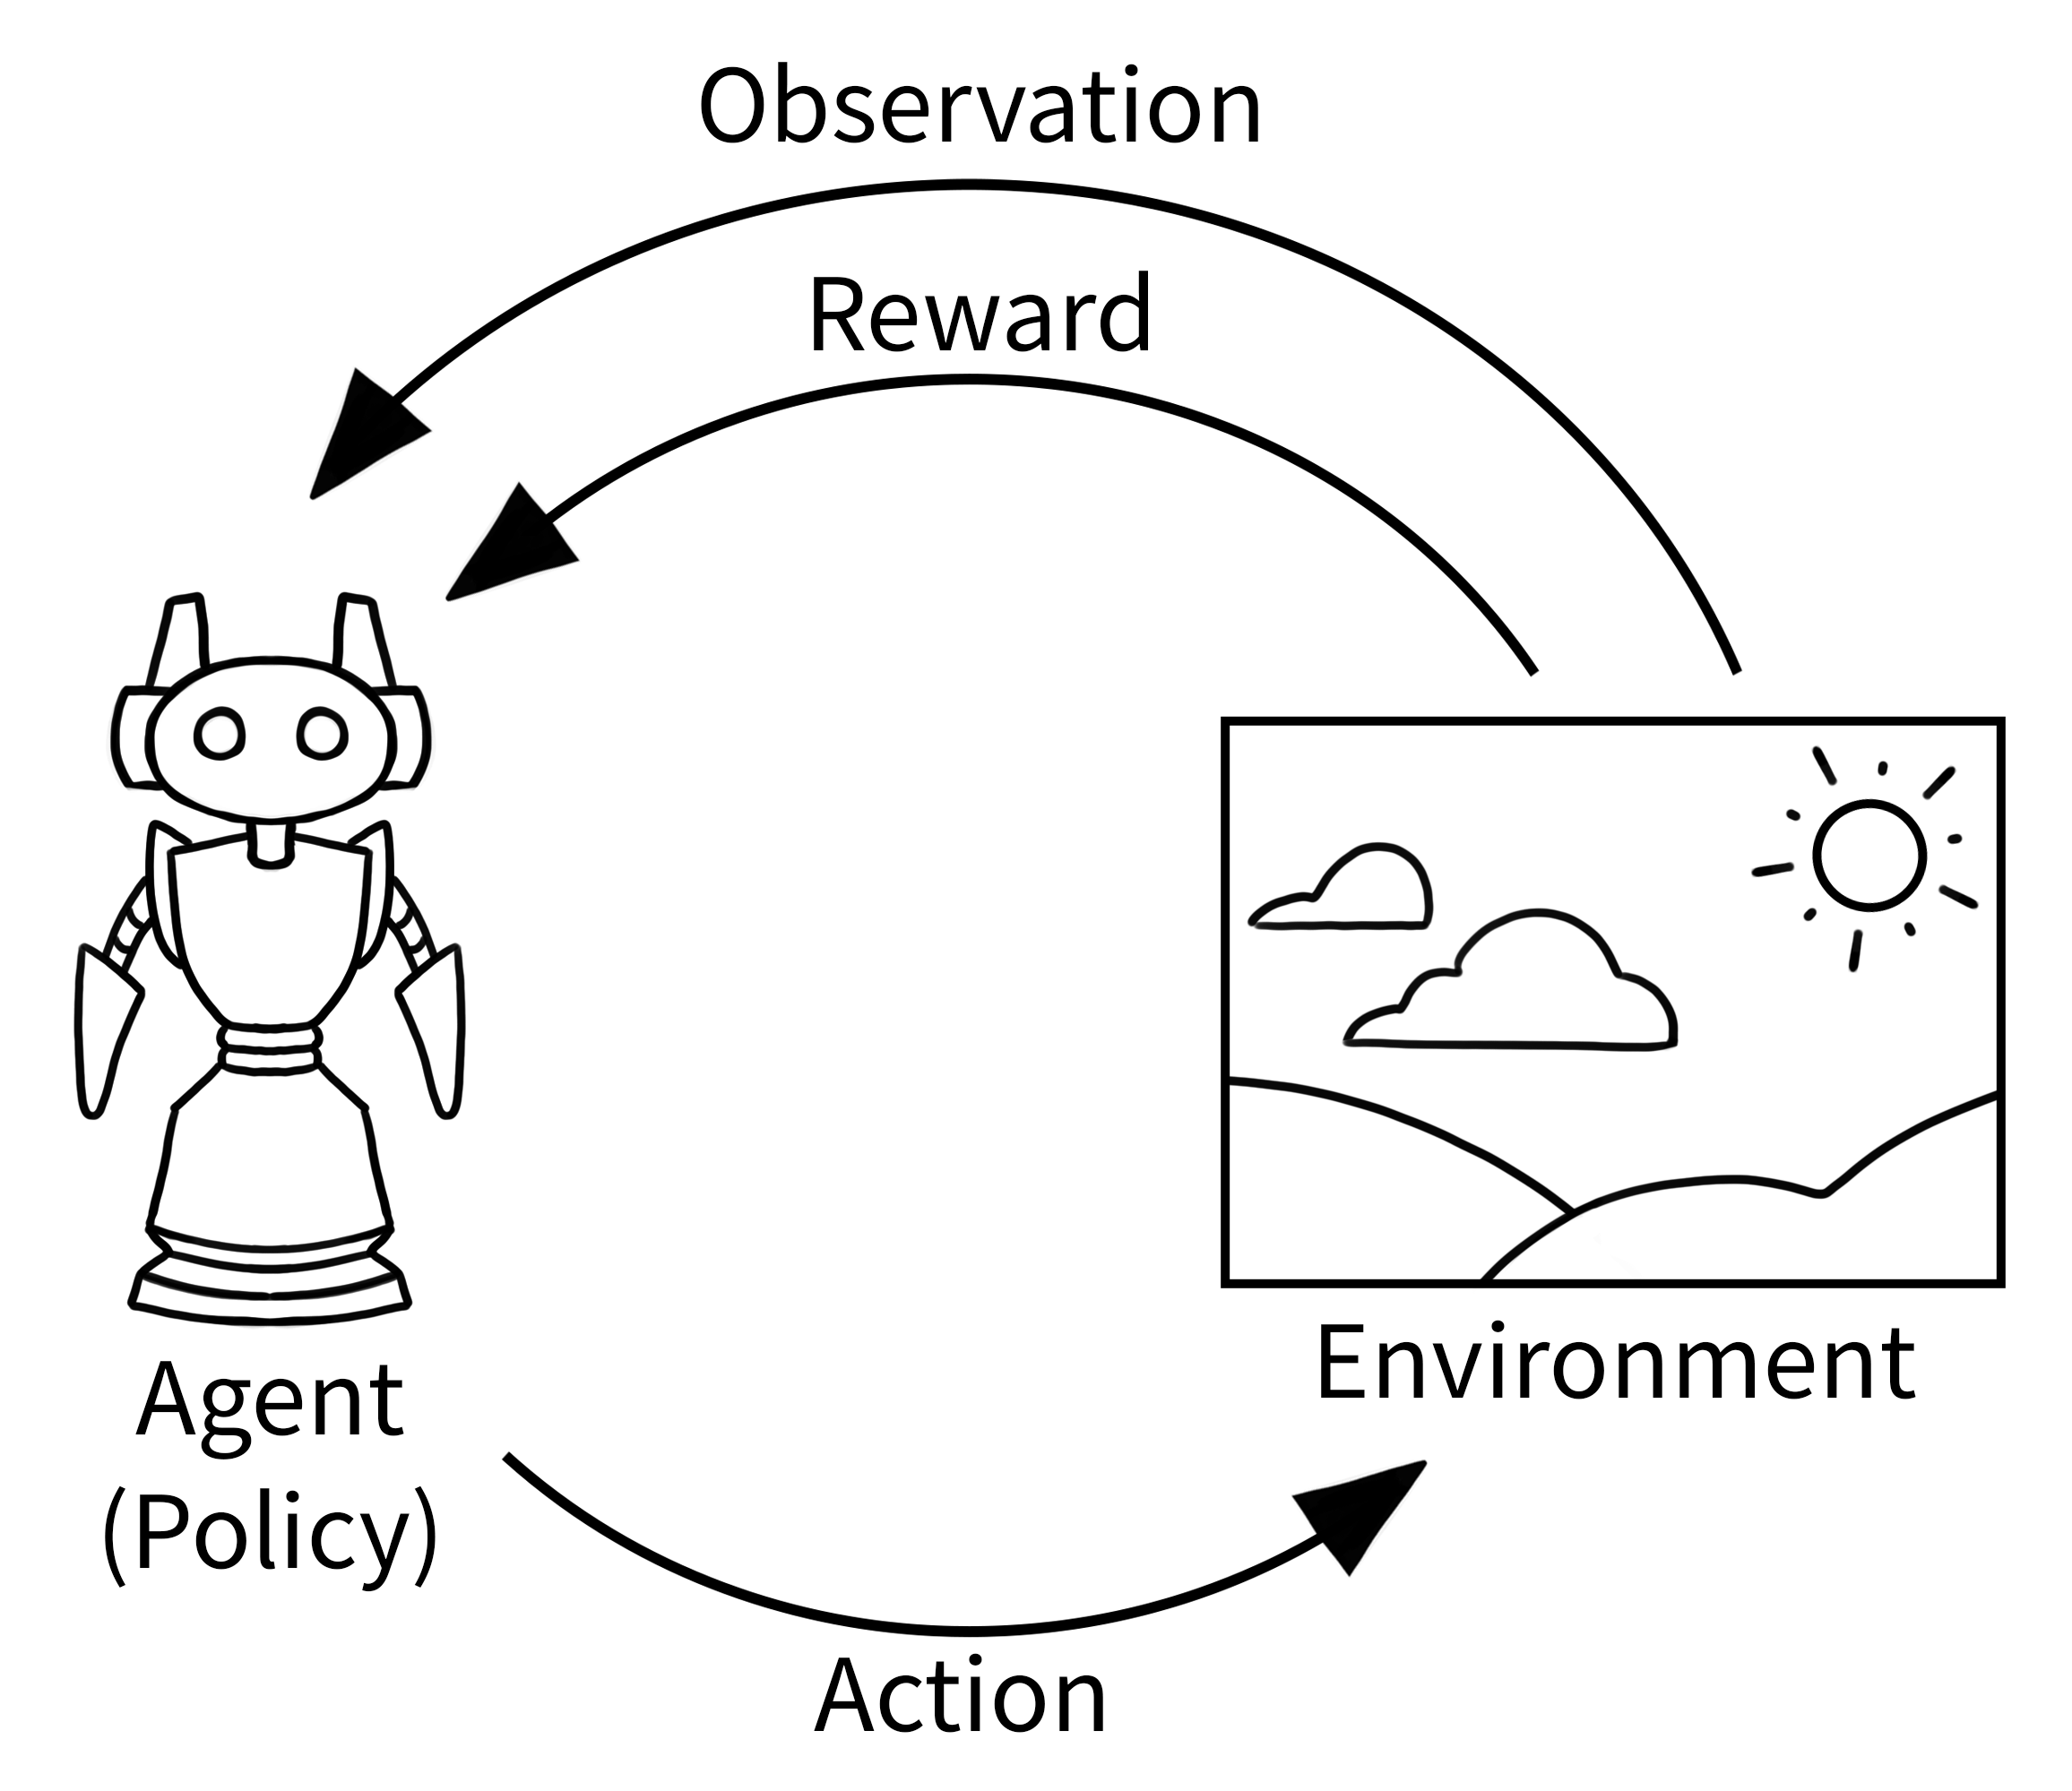
\includegraphics[width=\textwidth,height=0.6\textheight,keepaspectratio]{RL.png}
    \end{center}
\end{frame}
\begin{frame}[fragile]{Intro to Machine Learning}
    \textbf{Reinforcement Learning}
    \begin{itemize}
        \item is a machine learning system that learns to perform a task by interacting with its environment.
        \item has no supervisor signal.
        \item has delayed feedback.
        \item agent's actions affect future environments and the subsequent data.
        \item allows the agent to learn an optimal policy that maximizes long-term rewards.
    \end{itemize}
\end{frame}
\begin{frame}[fragile]{Intro to Machine Learning}
    \begin{center}
        \Huge Types of Machine Learning models
    \end{center}            
\end{frame}

\begin{frame}[fragile]{Intro to Machine Learning}
    \textbf{Types of Machine Learning models}\\
    \begin{itemize}
        \item By Model
        \item By Data
    \end{itemize}
\end{frame}

\begin{frame}[fragile]{Intro to Machine Learning}
    \textbf{By Model}\\
    ML models are categorised by how the model information is stored.
    \begin{itemize}
        \item Non-parametric models: All information, including training data, is stored within the model.
        \item Parametric models: Parametric models: Models store parameterised information derived from training data, including any specific parameter settings
    \end{itemize}
\end{frame}

\begin{frame}[fragile]{Intro to Machine Learning}
    \textbf{By Data}\\
    ML models are organised by the type of Data they interact with.
    \begin{center}
        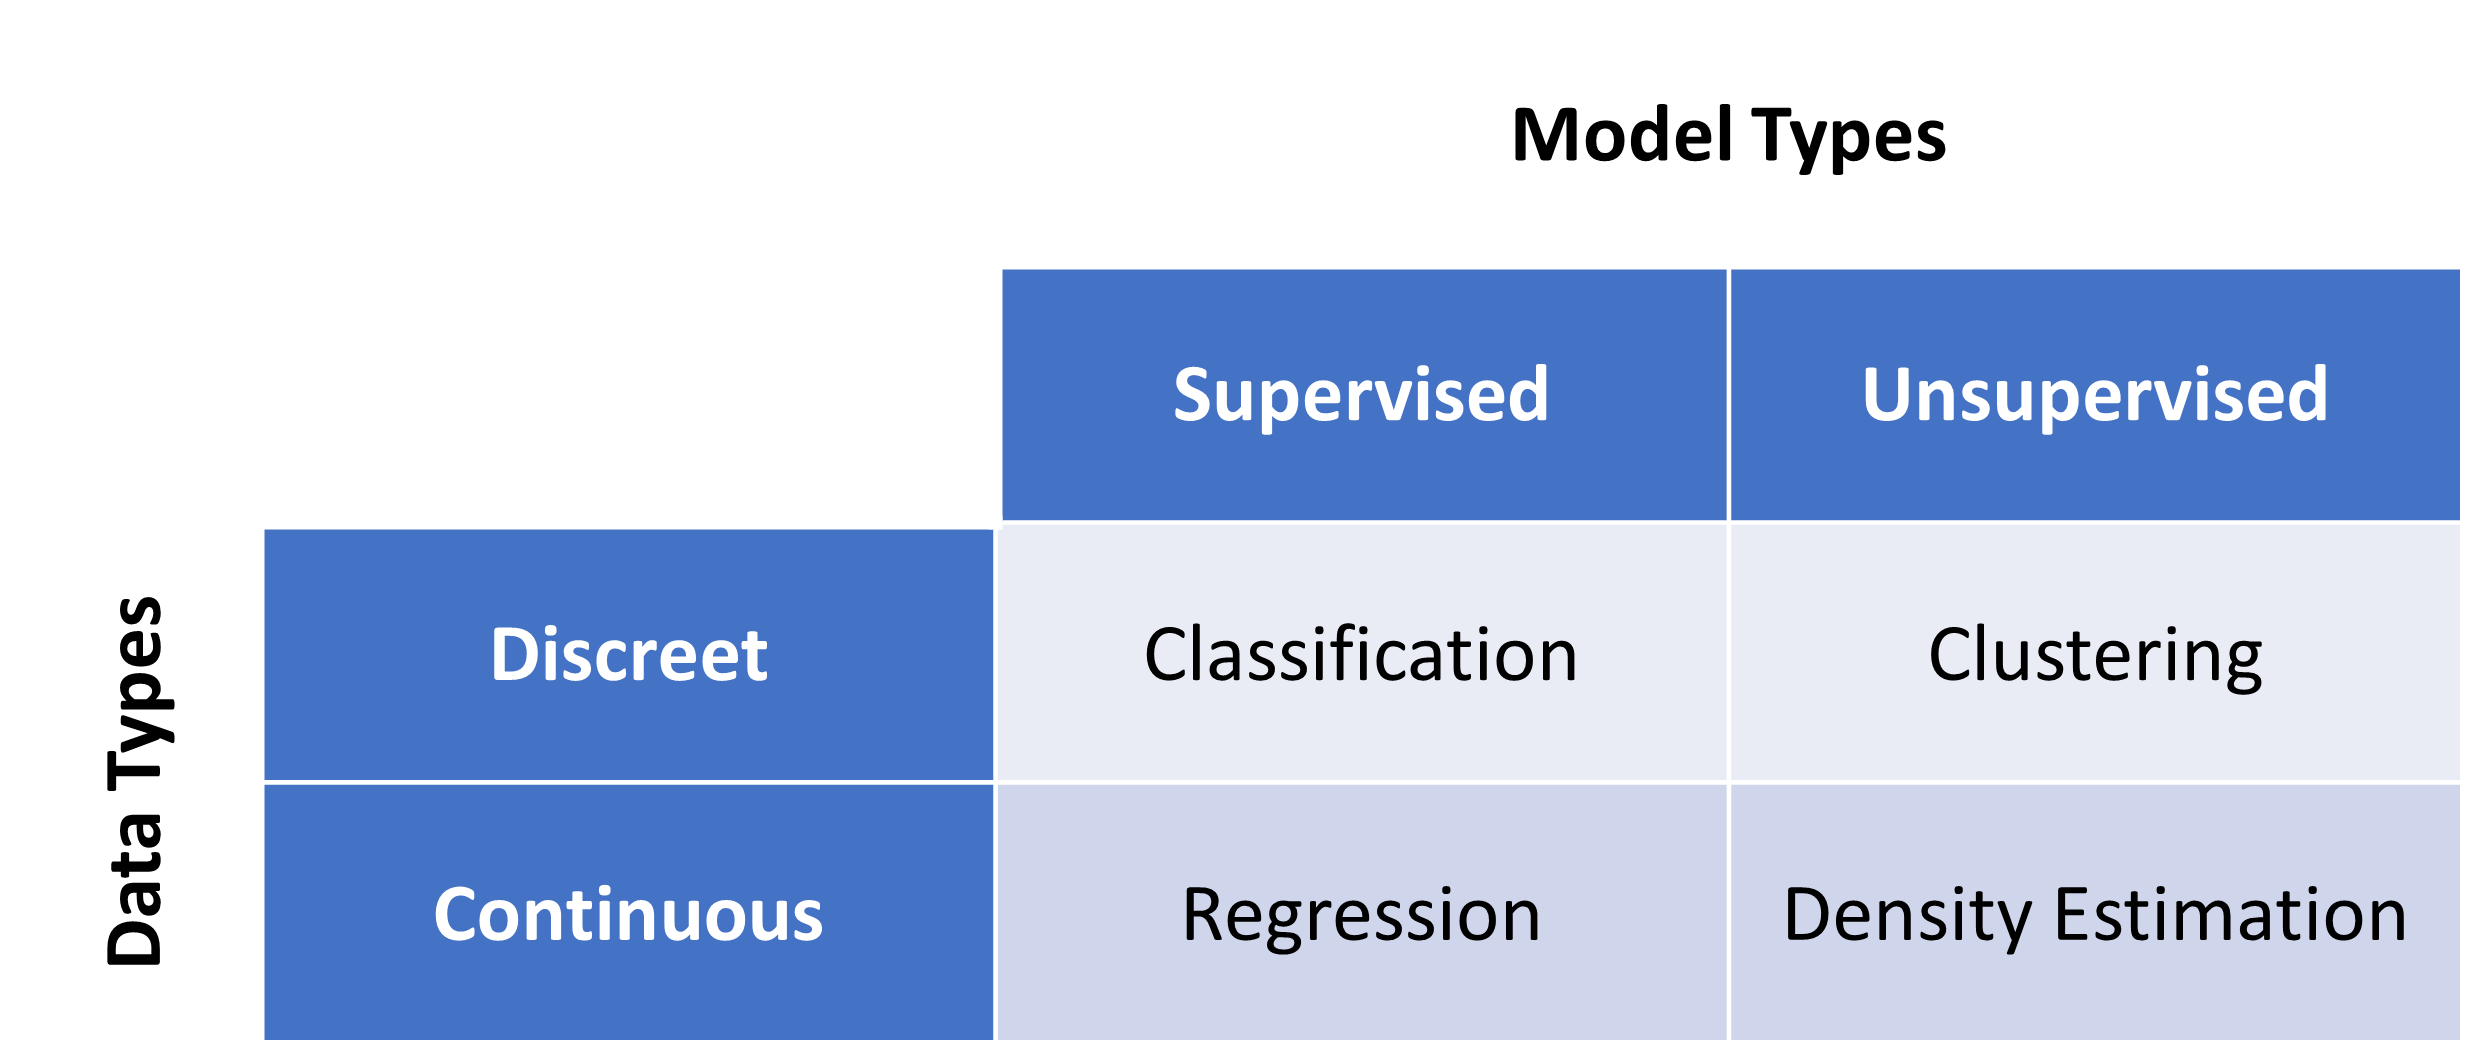
\includegraphics[width=\textwidth,height=\textheight,keepaspectratio]{By-Data.png}
    \end{center}
\end{frame}

\begin{frame}[fragile]{Types of Machine Learning}
    Generally, the domain of Machine Learning can be divided into two fields:
    \begin{itemize}
        \item Classical Machine Learning, where models rely on prior domain knowledge and hand-crafted features to function correctly.
        \item Contemporary Machine (Deep) Learning, where prior domain knowledge is optional, and models typically rely on feature extraction layers and deeper depth to function.
    \end{itemize}
\end{frame}
% 2 weeks
\subsection{Modelling Data with Classical Machine Learning}
\begin{frame}[fragile]{Classical Machine Learning}
    \vspace{-0.5cm}
    \textbf{Linear Models}
    \begin{block}{Definition}
        A model that describes the relationship between observations, $Y$, and input samples, $(X_1, X_2,..., X_p)$, as a weighted linear combination. Linear models assume that each input sample, $X_i$, is independent.
    \end{block}
    \vspace{-1cm}
    \begin{equation}
        y_i = w_0 + w_1 x_1 + w_2 x_2 + ... + w_p x_p
    \end{equation}
    Where $y_i$ is the $i$-th observation, $x_i$ is the $i$-th input sample, and $w_i$ is the weight.
    However, linear models are usually expressed in a full matrix form:
    \begin{equation}
        \label{eq:2}
        Y = XW^T + \epsilon
    \end{equation}
    where $Y$ is the matrix of observations, $X$ is the matrix of input samples, $W$ is the matrix of weights, and $\epsilon$ is the error term.
\end{frame}
\begin{frame}[fragile]{Classical Machine Learning}
    \textbf{Linear Regression}
    \href{https://scikit-learn.org/stable/modules/generated/sklearn.linear_model.LinearRegression.html}{\textbf{\underline{sklearn.linear\_model.LinearRegression}}}
    \begin{example}
        \begin{lstlisting}[language=Python]
from sklearn.linear_model import LinearRegression

reg = LinearRegression() # Initialise model
reg.fit(samples, targets) # Fit model to data
reg.predict(test_samples) # Make prediction
reg.score(test_samples, test_targets) # Evaluate
        \end{lstlisting}
    \end{example}
\end{frame}
\begin{frame}[fragile]{Classical Machine Learning}
    \textbf{Logistic Regression}
    \begin{block}{Definition}
        Logistic Regression is a discretized version of a linear regression model. To discretize the output, Logistic Regression uses sigmoid or softmax to map arbitrary numbers $\in \mathbb{R}$ to the [0, 1] range.
        \begin{columns}[T]
            \begin{column}{.40\textwidth}
                \begin{center}
                    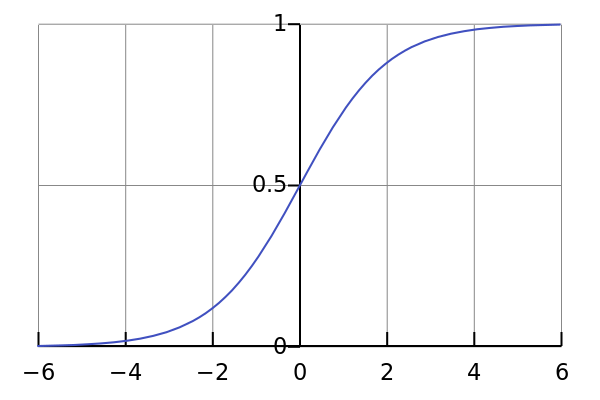
\includegraphics[width=.80\textwidth,height=\textheight,keepaspectratio]{Logistic-Sigmoid.png}
                \end{center}
            \end{column}%
            \hfill%
            \begin{column}{.40\textwidth}
                Sigmoid function:
                \begin{equation*}
                    \sigma(x) = \frac{1}{1 + \exp^{-x}}
                \end{equation*}
                Softmax function:
                \begin{equation*}
                    softmax(x)_{i} = \frac{\exp^{x_{i}}}{\sum_{j=1}^{K}\exp^{x_{j}}}
                \end{equation*}
            \end{column}%
        \end{columns}
    \end{block}
\end{frame}
\begin{frame}[fragile]{Classical Machine Learning}
    \textbf{Logistic Regression}
    \href{https://scikit-learn.org/stable/modules/generated/sklearn.linear_model.LogisticRegression.html}{\textbf{\underline{sklearn.linear\_model.LogisticRegression}}}
    \begin{example}
        \begin{lstlisting}[language=Python]
from sklearn.linear_model import LogisticRegression

clf = LogisticRegression(random_state=0) # Initialise model
clf.fit(samples, targets) # Fit model to data
clf.predict(test_samples) # Make prediction
clf.score(test_samples, test_targets) # Evaluate
        \end{lstlisting}
    \end{example}
\end{frame}
\begin{frame}[fragile]{Classical Machine Learning}
    \textbf{K-Mean clustering}
    \begin{block}{Definition}
        K-Mean is a clustering algorithm that tries to divide a set of $N$ samples into $K$ disjointed clusters of equal variance, each with centroid, $\mu_{i}$. To cluster the data, K-Mean places centroids at places that minimize:
        \vspace{-0.5cm}
        \begin{equation*}
            L(Cluster) = \sum_{i=0}^{n}\min\limits_{\mu_{j}\in C}(||x_{i} - \mu_{j}||^2)
        \end{equation*}
        where $C$ is the set of clusters.
        \begin{center}
            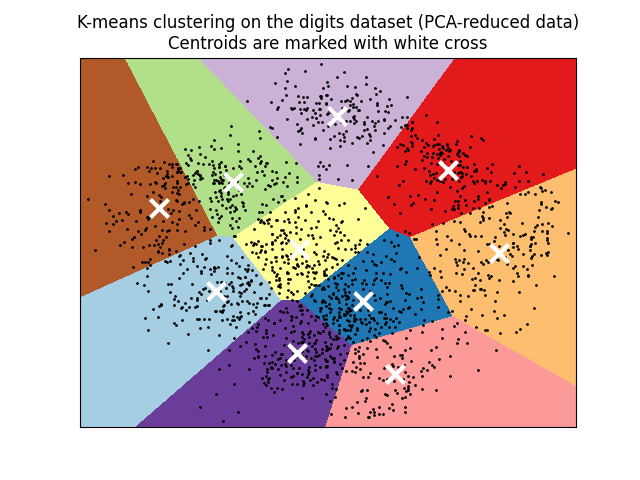
\includegraphics[width=.30\textwidth,height=\textheight,keepaspectratio]{k_mean.png}
        \end{center}
    \end{block}
\end{frame}
\begin{frame}[fragile]{Classical Machine Learning}
    \textbf{K-Mean clustering}
    \href{https://scikit-learn.org/stable/modules/generated/sklearn.cluster.KMeans.html}{\textbf{\underline{sklearn.cluster.KMeans}}}
    \begin{example}
        \begin{lstlisting}[language=Python]
from sklearn.cluster import KMeans

kmeans = KMeans(n_clusters=2, random_state=0, n_init="auto")
kmeans.fit(samples) # Fit model to data
kmeans.predict(test_samples) # Make prediction
        \end{lstlisting}
    \end{example}
\end{frame}

\begin{frame}[fragile]{Classical Machine Learning}
    \textbf{Principal component analysis}
    Similar to K-Mean, PCA is an unsupervised algorithm. However, unlike K-Mean, PCA operates on continuous variables to conduct dimensionality reduction. The principle of PCA is to decompose multivariate variables into a set of successive orthogonal components with a maximum amount of variance in each direction.
    \begin{center}
        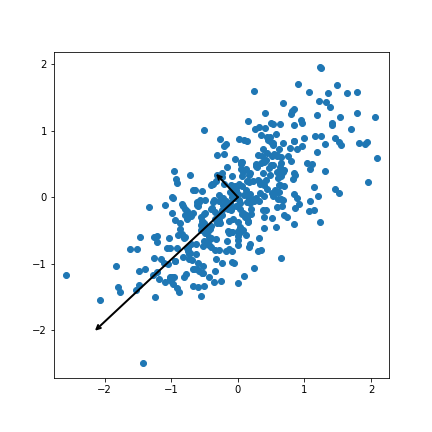
\includegraphics[width=.40\textwidth,height=\textheight,keepaspectratio]{PCA.png}
    \end{center}
\end{frame}
\begin{frame}[fragile]{Classical Machine Learning}
    \textbf{Principal component analysis}
    \href{https://scikit-learn.org/stable/modules/generated/sklearn.decomposition.PCA.html}{\textbf{\underline{sklearn.decomposition.PCA}}}
    \begin{example}
        \begin{lstlisting}[language=Python]
from sklearn.decomposition import PCA

pca = PCA(n_components=2)
pca.fit(samples) # Fit model to data
pca.transform(test_samples) # Decompose data
        \end{lstlisting}
    \end{example}
\end{frame}
\begin{frame}[fragile]{Classical Machine Learning}
    \textbf{Train-Test Split}
    One of the most common pitfalls in early-stage Machine Learning is training and evaluating the model on the same dataset, as the model would repeat previously seen connections between input samples and targeted observations, commonly known as overfitting. To truly assess the model's generalizability, the model must be evaluated on an unseen dataset, preferably in an adjacent distribution. To avoid overfitting, the dataset is usually split into training and testing sets.
    \begin{center}
        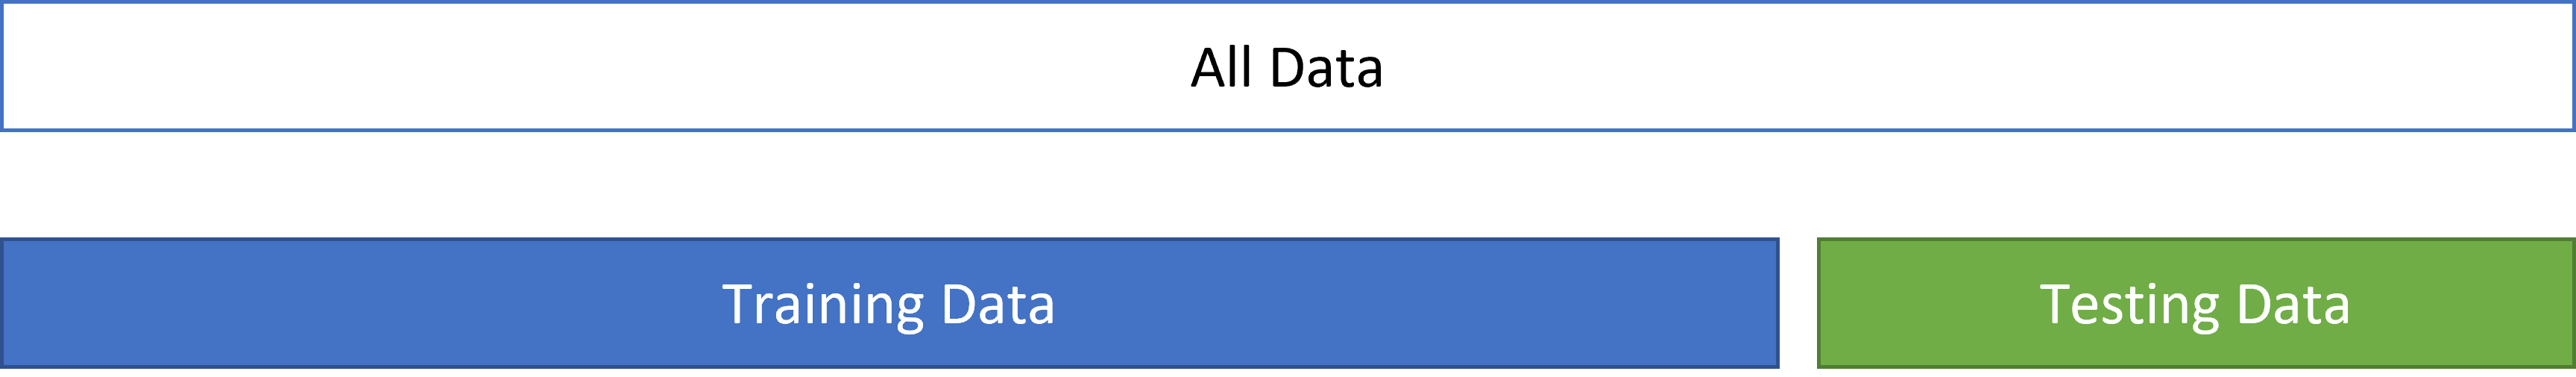
\includegraphics[width=\textwidth,height=\textheight,keepaspectratio]{Train-Test split.png}
    \end{center}
\end{frame}
\begin{frame}[fragile]{Classical Machine Learning}
    \textbf{Train-Test Split}
    \href{https://scikit-learn.org/stable/modules/generated/sklearn.model_selection.train_test_split.html}{\textbf{\underline{sklearn.model\_selection.train\_test\_split}}}
    \begin{example}
        \begin{lstlisting}[language=Python]
from sklearn.model_selection import train_test_split

# Split dataset into training and testing sets
X_train, X_test, y_train, y_test = train_test_split(
X, y, test_size=0.33,
random_state=42, shuffle=True)

# Split only input samples
X_train, X_test = train_test_split(X, shuffle=False)
        \end{lstlisting}
    \end{example}
\end{frame}
\begin{frame}[fragile]{Classical Machine Learning}
    \textbf{Cross-Validation}
    However, train-test splitting would only work if the overall dataset is large enough to provide enough training samples after the split and the data is evenly distributed. To overcome this problem, a procedure called K-Fold Cross-Validation can be used wherein the data set is partitioned into K, nearly identical size sub-datasets.
    \begin{center}
        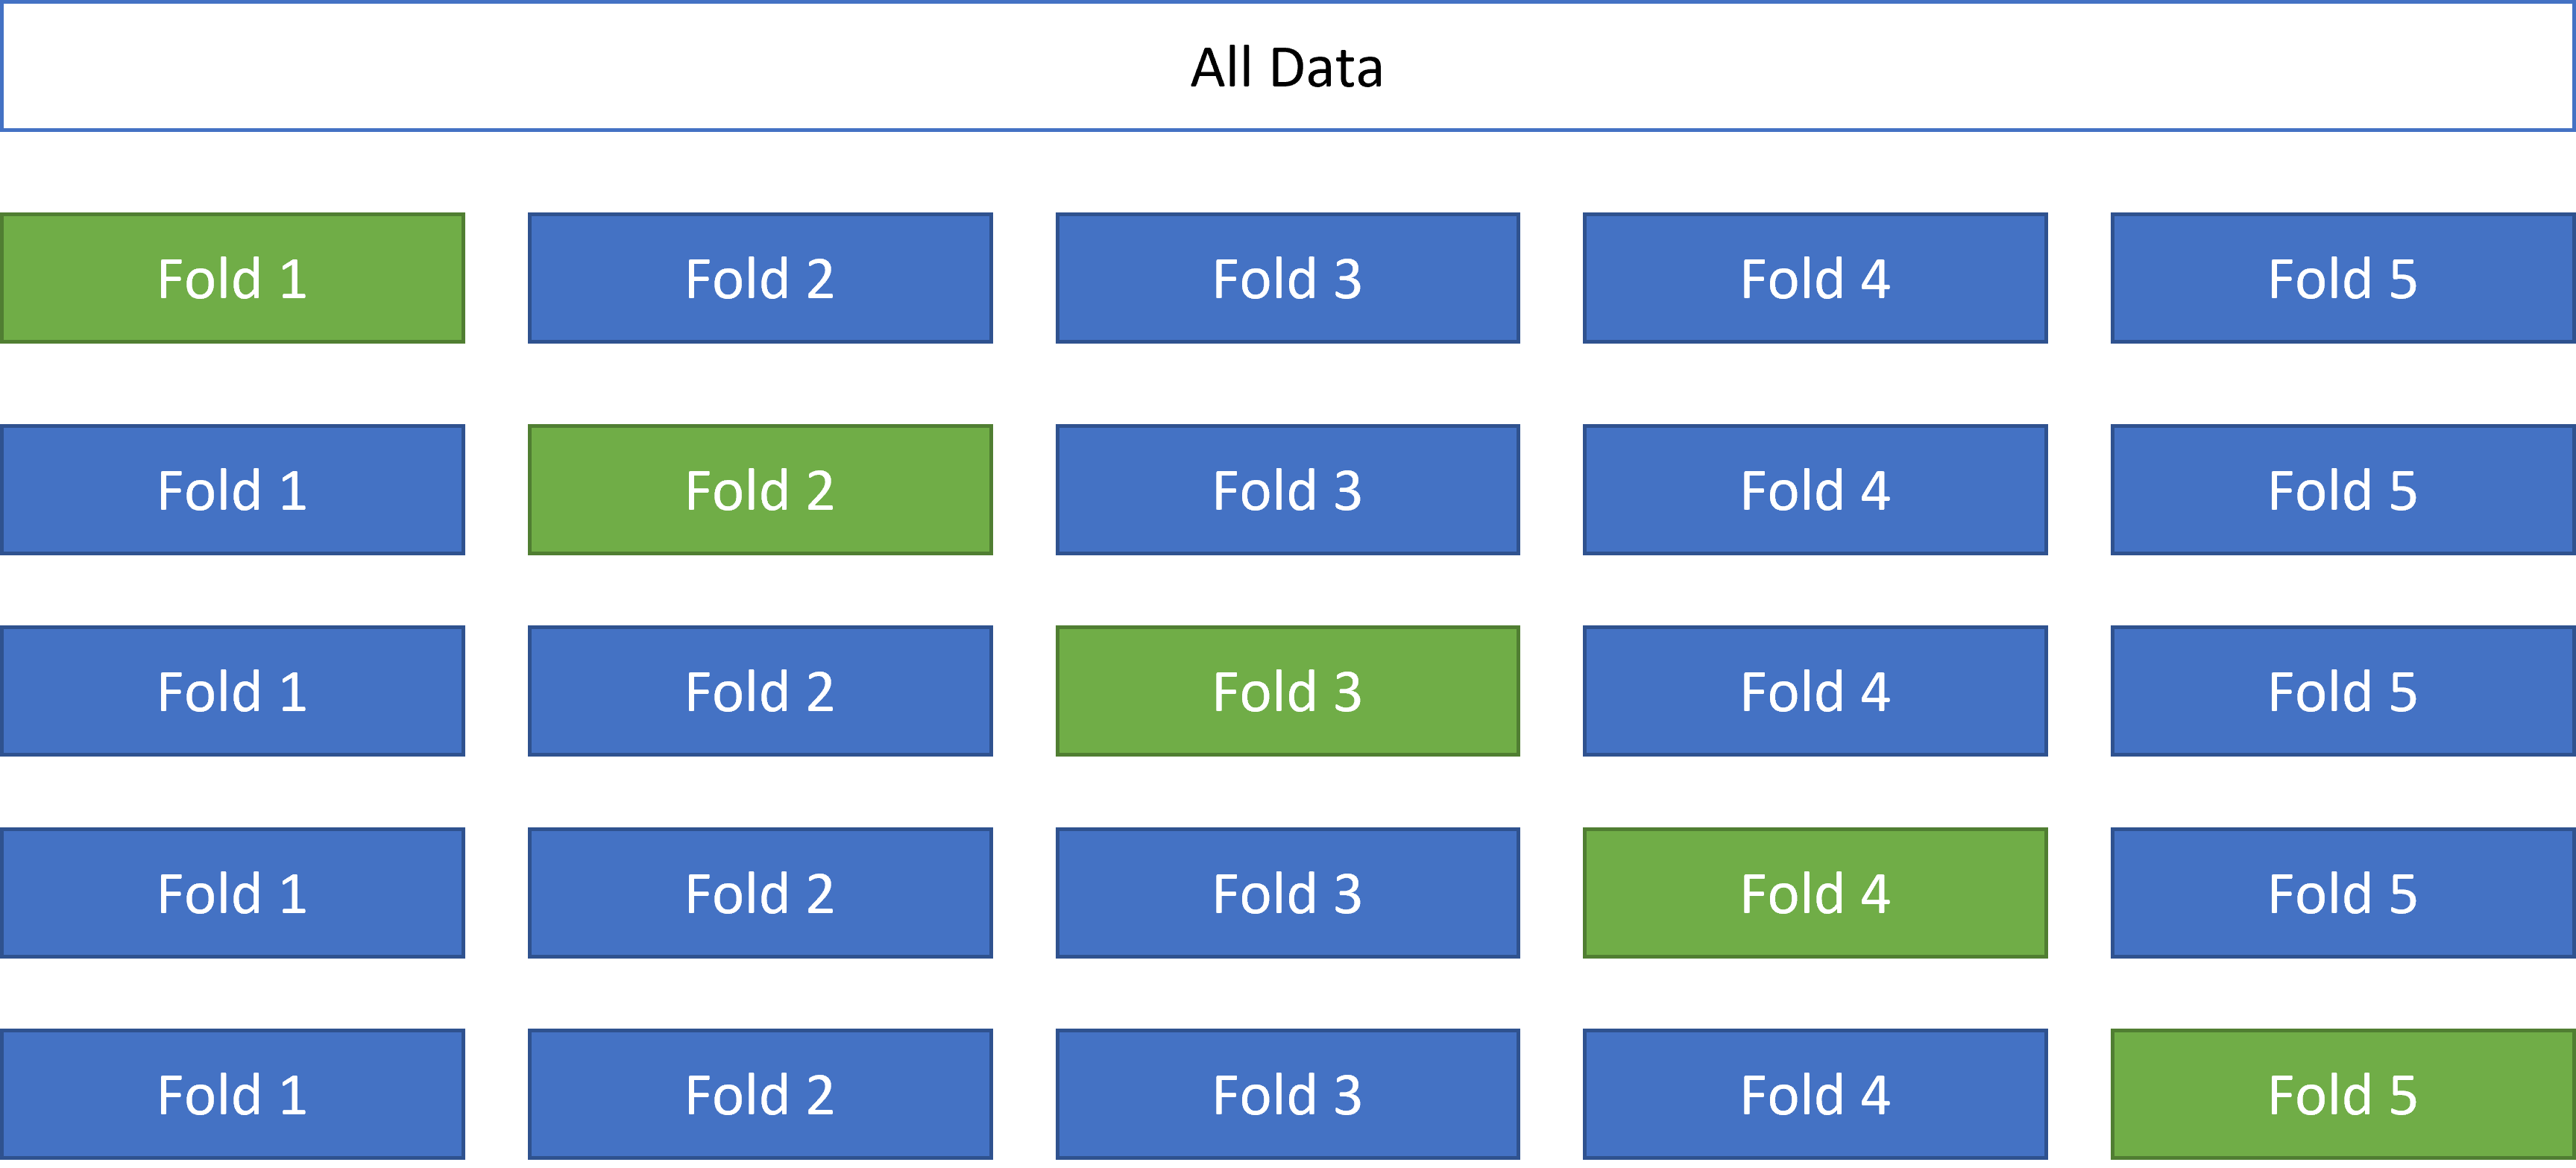
\includegraphics[width=0.8\textwidth,height=\textheight,keepaspectratio]{CV.png}
    \end{center}
\end{frame}
\begin{frame}[fragile]{Classical Machine Learning}
    \textbf{Cross-Validation}
    \href{https://scikit-learn.org/stable/modules/generated/sklearn.model_selection.cross_val_score.html}{\textbf{\underline{sklearn.model\_selection.cross\_val\_score}}}
    \begin{example}
        \begin{lstlisting}[language=Python]
from sklearn.model_selection import cross_val_score

# Load dataset
X, y = load_dataset()

# Build model
model = build_model()

# CV scores
cv_scores = cross_val_score(model, X, y, cv=5)
        \end{lstlisting}
    \end{example}
\end{frame}
\end{document}